% Optimized by ChatGPT: improved title area, margins, frametitle, figure sizing, callouts.
\PassOptionsToPackage{pdfpagelabels=false}{hyperref}
\documentclass[aspectratio=169,10pt]{ctexbeamer}

\usepackage{booktabs}
\usepackage{array}
\usepackage{graphicx}
\usepackage{tikz}
\usepackage{amsmath}
\usepackage{microtype}
\usepackage{bookmark}
\usetikzlibrary{arrows.meta,positioning,fit,calc,matrix,backgrounds}

\graphicspath{
  {../paper/figs/}
  {../paper/out/}
  {../paper/resources/}
  {paper/figs/}
  {paper/out/}
  {paper/resources/}
}

\definecolor{ink}{HTML}{17212B}
\definecolor{muted}{HTML}{64748B}
\definecolor{line}{HTML}{CBD5E1}
\definecolor{soft}{HTML}{F5F7FA}
\definecolor{blue}{HTML}{2563EB}
\definecolor{teal}{HTML}{0F766E}
\definecolor{red}{HTML}{DC2626}
\definecolor{amber}{HTML}{B45309}
\definecolor{violet}{HTML}{6D28D9}
\definecolor{green}{HTML}{15803D}

\setbeamertemplate{navigation symbols}{}
\usefonttheme{professionalfonts}
\setbeamersize{text margin left=0.68cm,text margin right=0.68cm}

\setbeamertemplate{frametitle}{%
  \vspace{0.18cm}%
  \begin{beamercolorbox}[wd=\paperwidth,ht=0.58cm,leftskip=0.68cm,rightskip=0.42cm]{frametitle}
    \usebeamerfont{frametitle}\insertframetitle
    \ifx\insertpaperref\empty\else\hfill\insertpaperref\fi
  \end{beamercolorbox}%
  \vspace{0.08cm}%
}
\setbeamertemplate{footline}{
  \hfill
  \scriptsize\color{muted}\insertframenumber/\inserttotalframenumber
  \hspace{0.42cm}\vspace{0.18cm}
}
\setbeamercolor{normal text}{fg=ink,bg=white}
\setbeamercolor{frametitle}{fg=ink,bg=white}
\setbeamerfont{frametitle}{series=\bfseries,size=\Large}
\setbeamerfont{title}{series=\bfseries,size=\LARGE}
\setlength{\parskip}{1.5pt}
\setlength{\abovedisplayskip}{5pt}
\setlength{\belowdisplayskip}{5pt}

\tikzset{
  box/.style={
    draw=line, fill=soft, rounded corners=2pt,
    inner xsep=6pt, inner ysep=5pt,
    align=center, font=\small
  },
  pill/.style={
    rounded corners=2pt, inner xsep=7pt, inner ysep=3.5pt,
    font=\small\bfseries, text=white
  },
  arrow/.style={-{Latex[length=2.2mm]}, thick, draw=muted},
  thinarr/.style={-{Latex[length=1.8mm]}, draw=muted},
  metric/.style={
    draw=line, rounded corners=1.5pt,
    inner xsep=6pt, inner ysep=6pt,
    align=center, font=\small, fill=white
  }
}

\newcommand{\tagpill}[2]{%
  \tikz[baseline=(x.base)]\node[pill,fill=#1](x){#2};%
}
\newcommand{\metricbox}[3]{%
  \begin{tikzpicture}
    \node[metric, minimum width=0.29\linewidth] {
      {\Large\bfseries #1}\\[-1pt]
      {\footnotesize #2}\\[-1pt]
      {\scriptsize\color{muted}#3}
    };
  \end{tikzpicture}%
}
\newcommand{\tinymetric}[3]{%
  \begin{tikzpicture}
    \node[metric, minimum width=0.30\linewidth, inner xsep=4pt, inner ysep=5pt] {
      {\large\bfseries #1}\\[-1pt]
      {\scriptsize #2}\\[-1pt]
      {\tiny\color{muted}#3}
    };
  \end{tikzpicture}%
}

\newcommand{\slidelead}[1]{%
  {\small\color{muted}#1}\par\vspace{0.18cm}%
}
\let\insertpaperref\empty
\let\nextpaperref\empty
\newcommand{\paperref}[1]{%
  \gdef\nextpaperref{#1}%
}
\BeforeBeginEnvironment{frame}{%
  \global\let\insertpaperref\nextpaperref
  \global\let\nextpaperref\empty
}
\newcommand{\imagefit}[2][]{%
  \includegraphics[width=\linewidth,height=#2,keepaspectratio,#1]%
}
\newcommand{\captionline}[1]{%
  \vspace{0.04cm}\centering{\scriptsize\color{muted}#1}%
}
\newcommand{\formularow}[4]{%
  {\setbeamercolor{formulaPanel}{fg=ink,bg=#1}%
  \begin{beamercolorbox}[wd=\linewidth,sep=5.2pt,rounded=true]{formulaPanel}
    \scriptsize
    \begin{tabular}{@{}>{\raggedright\arraybackslash}m{0.15\linewidth}@{\hspace{0.012\linewidth}}>{\centering\arraybackslash}m{0.72\linewidth}@{\hspace{0.012\linewidth}}>{\raggedleft\arraybackslash}m{0.08\linewidth}@{}}
      \bfseries #2 &
      $\displaystyle #3$ &
      {\color{muted}\bfseries (#4)}
    \end{tabular}
  \end{beamercolorbox}}%
}
\newcommand{\formulagap}{\vspace{0.14cm}}

\newcommand{\algpreview}[1]{%
  \includegraphics[
    page=#1,
    width=\linewidth,
    height=0.74\textheight,
    keepaspectratio,
    trim=0.8cm 13.0cm 0.8cm 0.6cm,
    clip
  ]{core_algorithm_tikz_preview.pdf}%
}

\title{基于领域自适应的\\工业过程故障诊断方法研究}
\subtitle{答辩汇报}
\author{08022311 陈鲲龙}
\institute{东南大学自动化学院}
\date{2026年6月}

\begin{document}

\begin{frame}[plain,noframenumbering]
  \begingroup
  \setlength{\parindent}{0pt}
  \vspace*{0.44cm}
  \begin{minipage}[t]{0.62\textwidth}
    \raisebox{0.46cm}[0pt][0pt]{\color{muted}\large 本科毕业设计答辩}
  \end{minipage}
  \hfill
  \begin{minipage}[t]{0.28\textwidth}
    \raggedleft
\includegraphics[width=2.78cm]{seu-text-logo.png}
  \end{minipage}

  \vspace{0.52cm}
  {\fontsize{23}{27}\selectfont\bfseries 基于领域自适应的\\工业过程故障诊断方法研究\par}

  \vspace{0.46cm}
  {\fontsize{15.8}{19}\selectfont 面向 TEP 数据集的无监督领域自适应故障诊断\par}

  \vspace{0.58cm}
  \begin{tikzpicture}
    \node[
      draw=line,
      fill=soft,
      rounded corners=2pt,
      minimum width=7.95cm,
      anchor=west,
      inner xsep=0.38cm,
      inner ysep=0.22cm,
      align=left
    ] at (0,0) {%
      {%
      \renewcommand{\arraystretch}{1.28}%
      \begin{tabular}{@{}l@{\hspace{0.17cm}}l@{}}
        {\large\bfseries\strut 08022311} & {\large\bfseries\strut 陈鲲龙}\\
        {\large\strut 指导教师：} & {\large\strut 王永健}\\
        \multicolumn{2}{@{}l@{}}{\large\strut 自动化学院}\\
        \multicolumn{2}{@{}l@{}}{\large\strut 2026.6}
      \end{tabular}%
      }%
    };
  \end{tikzpicture}
  \endgroup
\end{frame}

\paperref{P40}
\begin{frame}{研究问题界定：TE过程无监督领域自适应故障诊断}
  \slidelead{聚焦 TE 过程及其数据集，将领域自适应故障诊断定义为无监督跨工况自适应问题。}
  \begin{columns}[T,totalwidth=\textwidth]
    \begin{column}{0.57\textwidth}
      \vspace{0.28cm}
      \resizebox{\linewidth}{!}{%
      \begin{tikzpicture}
        \node[font=\footnotesize\color{muted}, align=center] at (-2.75,1.64)
          {源域有标签样本可用};
        \node[font=\footnotesize\color{muted}, align=center] at (2.75,1.64)
          {目标域标签不参与算法};
        \node[box, fill=blue!6, draw=blue!30, minimum width=3.15cm, minimum height=1.25cm] (src) at (-2.75,0.56)
          {源域工况\\{\footnotesize 单源或多源}\\{\footnotesize 标签参与训练}};
        \node[box, fill=red!5, draw=red!28, minimum width=3.15cm, minimum height=1.25cm] (tgt) at (2.75,0.56)
          {目标域工况\\{\footnotesize 单目标}\\{\footnotesize 训练时无标签}};
        \node[box, fill=teal!6, draw=teal!30, minimum width=3.25cm, minimum height=1.25cm] (model) at (0,-1.22)
          {诊断模型\\{\footnotesize 特征提取}\\{\footnotesize 状态分类}};
        \draw[arrow] (src.south) |- (model.west);
        \draw[arrow] (tgt.south) |- (model.east);
        \node[box, below=0.82cm of model, minimum width=4.35cm, fill=green!7, draw=green!32] (pred)
          {目标域分类状态预测\\{\footnotesize 评价目标：准确率尽可能高}};
        \draw[arrow] (model) -- (pred);
      \end{tikzpicture}
      }
    \end{column}
    \begin{column}{0.39\textwidth}
      \vspace{0.02cm}
      \begin{tikzpicture}[node distance=0.24cm]
        \node[box, anchor=west, fill=white, minimum width=4.65cm, text width=4.25cm, align=left] (data)
          {\textbf{TEP 数据集}\\{\footnotesize 6 个工况 $\rightarrow$ 6 个领域}\\{\footnotesize 0 正常 + 1--28 类故障 $\rightarrow$}\\{\footnotesize 29 个分类状态}};
        \node[box, anchor=west, fill=blue!6, draw=blue!30, minimum width=4.65cm, text width=4.25cm, align=left, below=of data] (task)
          {\textbf{单源 / 多源 $\rightarrow$ 单目标}\\{\footnotesize 源域监督，目标域无监督训练}};
        \node[box, anchor=west, fill=teal!6, draw=teal!30, minimum width=4.65cm, text width=4.25cm, align=left, below=of task] (label)
          {\textbf{训练约束}\\{\footnotesize 目标域标签不参与算法}};
        \node[box, anchor=west, fill=green!7, draw=green!32, minimum width=4.65cm, text width=4.25cm, align=left, below=of label] (goal)
          {\textbf{目标}\\{\footnotesize 提高目标域 29 类状态诊断准确率}};
      \end{tikzpicture}
    \end{column}
  \end{columns}
\end{frame}

\paperref{P7}
\begin{frame}{核心成果：3套创新算法}
  \centering
  \vspace*{\fill}
  \resizebox{0.76\textwidth}{!}{%
  \begin{tikzpicture}
    \node[box, fill=white, minimum width=2.35cm] (deep) at (-3.55,0) {DeepJDOT};
    \node[box, fill=blue!8, draw=blue!40, minimum width=3.45cm, text width=3.18cm] (tpu) at (0,0)
      {\textbf{TPU-DeepJDOT}\\{\scriptsize\bfseries 时序原型非平衡\\联合分布对齐}};
    \node[box, fill=teal!8, draw=teal!40, minimum width=3.45cm, text width=3.18cm] (cbtpu) at (4.05,0)
      {\textbf{CBTPU-DeepJDOT}\\{\scriptsize\bfseries 多证据置信\\均衡伪标签}};
    \node[box, fill=red!6, draw=red!35, text=red, font=\small\bfseries, minimum width=2.55cm] (riskmatch) at (0,1.42)
      {错误匹配};
    \node[box, fill=red!6, draw=red!35, text=red, font=\small\bfseries, minimum width=2.55cm] (riskpseudo) at (4.05,1.42)
      {伪标签噪声};
    \draw[arrow] (deep) -- (tpu);
    \draw[arrow] (tpu) -- (cbtpu);
    \draw[thinarr, draw=red!45] (riskmatch.south) -- (tpu.north);
    \draw[thinarr, draw=red!45] (riskpseudo.south) -- (cbtpu.north);
    \node[font=\footnotesize\color{muted}, align=center] (single) at (2.02,-1.02)
      {单源：先建立可靠对齐，再谨慎利用目标样本};

    \node[box, fill=white, minimum width=2.35cm] (wj) at (-3.55,-3.20) {WJDOT};
    \node[box, fill=amber!10, draw=amber!45, minimum width=3.45cm] (codats) at (0,-3.20)
      {CoDATS 表征};
    \node[box, fill=violet!8, draw=violet!40, minimum width=3.45cm, text width=3.18cm] (ca) at (4.05,-3.20)
      {\textbf{CA-CCSR-WJDOT}\\{\scriptsize\bfseries 类条件源域\\可靠性加权}};
    \node[box, fill=red!6, draw=red!35, text=red, font=\small\bfseries, minimum width=2.55cm] (riskmulti) at (4.05,-1.78)
      {多源负迁移};
    \draw[arrow] (wj) -- (codats);
    \draw[arrow] (codats) -- (ca);
    \draw[thinarr, draw=red!45] (riskmulti.south) -- (ca.north);
    \node[font=\footnotesize\color{muted}, align=center] (multi) at (2.02,-4.36)
      {多源：不合并为一个大源域，改为类别级加权};

    \begin{pgfonlayer}{background}
      \node[draw=amber!35, fill=amber!5, fill opacity=0.55, rounded corners=2pt,
        inner xsep=10pt, inner ysep=8pt,
        fit=(riskmatch)(riskpseudo)(tpu)(cbtpu)(single)(riskmulti)(codats)(ca)(multi)] {};
    \end{pgfonlayer}
  \end{tikzpicture}
  }
  \vspace*{\fill}
\end{frame}

\paperref{P16}
\begin{frame}{方法一：TPU-DeepJDOT 架构}
  \centering
  \vspace*{\fill}
  \resizebox{!}{0.865\textheight}{\begin{tikzpicture}[
    x=1cm,
    y=1.35cm,
    >=stealth,
    font=\small\fontspec{Times New Roman}\songti,
    card/.style={
        draw,
        rounded corners=4pt,
        line width=0.45pt,
        fill=white
    },
    chip/.style={
        draw,
        rounded corners=2pt,
        line width=0.35pt,
        fill=white,
        align=center,
        inner xsep=5pt,
        inner ysep=5pt
    },
    bluecard/.style={card, draw=blue!45!black, fill=blue!4},
    cyancard/.style={card, draw=cyan!50!black, fill=cyan!5},
    orangecard/.style={card, draw=orange!65!black, fill=orange!6},
    greencard/.style={card, draw=green!45!black, fill=green!6},
    redcard/.style={card, draw=red!45!black, fill=red!5},
    panel/.style={draw=black!15, rounded corners=5pt, line width=0.35pt, fill=gray!1},
    arrow/.style={->, line width=0.55pt, draw=black!70},
    note/.style={font=\scriptsize\fontspec{Times New Roman}\songti, align=center}
]

\draw[panel] (-0.25,0.00) rectangle (17.95,9.00);
\node[font=\large\fontspec{Times New Roman}\songti] at (8.85,8.55)
    {TPU-DeepJDOT 时序原型非平衡联合分布对齐机制};

% 输入批次
\draw[bluecard] (0.55,2.15) rectangle (3.25,7.75);
\node at (1.90,7.43) {输入批次};
\node[chip, minimum width=2.05cm] at (1.90,6.05)
    {源域有标签\\[-1pt]$\mathcal{B}_s$};
\node[chip, minimum width=2.05cm] at (1.90,4.60)
    {目标域无标签\\[-1pt]$\mathcal{B}_t$};
\node[note, text width=2.20cm] at (1.90,3.25)
    {训练阶段不使用目标标签};

% 时序诊断网络
\draw[cyancard] (4.05,2.15) rectangle (7.55,7.75);
\node at (5.80,7.43) {时序诊断网络};
\node[chip, minimum width=2.60cm] at (5.80,6.05)
    {共享 FCN 表征\\[-1pt]$z=F_\theta(x)$};
\node[chip, minimum width=2.60cm] at (5.80,4.60)
    {诊断分类器\\[-1pt]$p=G_\phi(z)$};
\node[note, text width=2.75cm] at (5.80,3.25)
    {源域监督形成基础判别边界};

% 结构增强约束
\draw[orangecard] (8.35,2.15) rectangle (11.95,7.75);
\node at (10.15,7.43) {结构增强约束};
\node[chip, minimum width=2.75cm] at (10.15,6.25)
    {源域类别原型\\[-1pt]$\mu_c,\ r_{ij}^{\mathrm{proto}}$};
\node[chip, minimum width=2.75cm] at (10.15,4.95)
    {时序统计描述符\\[-1pt]$\psi(x),\ c_{ij}^{\mathrm{temp}}$};
\node[chip, minimum width=2.75cm] at (10.15,3.65)
    {源域监督对比\\[-1pt]$\mathcal{L}_{\mathrm{supcon}}$};
\node[note, text width=2.90cm] at (10.15,2.60)
    {修正传输代价，预热源类结构};

% 非平衡联合传输
\draw[greencard] (12.75,2.15) rectangle (17.25,7.75);
\node at (15.00,7.43) {非平衡联合传输};
\node[chip, minimum width=3.35cm] at (15.00,6.25)
    {联合代价矩阵\\[-1pt]$C_{ij}$};
\node[chip, minimum width=3.35cm] at (15.00,4.95)
    {非平衡 Sinkhorn\\[-1pt]$\gamma^\ast,\tau_s,\tau_t$};
\node[chip, minimum width=3.35cm] at (15.00,3.65)
    {对齐损失\\[-1pt]$\mathcal{L}_{\mathrm{align}}$};
\node[note, text width=3.35cm] at (15.00,2.60)
    {边际质量可削减，缓解错误强制匹配};

% 优化目标
\draw[redcard] (4.05,0.50) rectangle (17.25,1.35);
\node at (10.65,0.92)
    {$\mathcal{L}_{\mathrm{TPU}}
    =\mathcal{L}_{\mathrm{src}}
    +\lambda_{\mathrm{supcon}}\mathcal{L}_{\mathrm{supcon}}
    +\lambda_{\mathrm{ot}}\mathcal{L}_{\mathrm{align}}$};

\draw[arrow] (3.25,4.95) -- (4.05,4.95);
\draw[arrow] (7.55,4.95) -- (8.35,4.95);
\draw[arrow] (11.95,4.95) -- (12.75,4.95);
\draw[arrow] (15.00,2.15) -- (15.00,1.35);

\end{tikzpicture}
}
  \vspace*{\fill}
\end{frame}

\paperref{P19}
\begin{frame}{方法一：联合代价与非平衡传输}
  \vspace*{0.22cm}
  \formularow{blue!4}{联合代价}{
    C_{ij}=\lambda_f c^f_{ij}+\lambda_y c^y_{ij}
    +\lambda_p(\nu)r_{ij}^{\mathrm{proto}}
    +\lambda_{\mathrm{temp}}(\nu)c_{ij}^{\mathrm{temp}}
  }{3-13}
  \formulagap
  \formularow{amber!5}{原型惩罚}{
    r_{ij}^{\mathrm{proto}}=\operatorname{clip}\!\left(
    \frac{d_{y_i^s j}^{\mathrm{proto}}-\overline d_{-y_i^s,j}^{\mathrm{proto}}}
    {\sigma_j^{\mathrm{proto}}+\epsilon},r_{\min},r_{\max}\right)
  }{3-7}
  \formulagap
  \formularow{violet!5}{时序代价}{
    c_{ij}^{\mathrm{temp}}=\frac{1}{d_\psi}\|\psi(x_i^s)-\psi(x_j^t)\|_2^2
  }{3-11}
  \formulagap
  \formularow{green!5}{总目标}{
    \mathcal{L}_{\mathrm{TPU}}=\mathcal{L}_{\mathrm{src}}
    +\lambda_{\mathrm{supcon}}(\nu)\mathcal{L}_{\mathrm{supcon}}
    +\lambda_{\mathrm{ot}}(\nu)\mathcal{L}_{\mathrm{align}}
  }{3-20}
\end{frame}

\paperref{P21}
\begin{frame}{方法一：TPU-DeepJDOT 训练流程}
  \begin{columns}[c,onlytextwidth,totalwidth=\textwidth]
    \begin{column}{0.58\textwidth}
      \centering
      \resizebox{\linewidth}{!}{%
      \begin{tikzpicture}[node distance=0.42cm]
        \node[box, fill=blue!7, draw=blue!35, minimum width=2.55cm] (a) {采样批次\\源有标签 / 目标无标签};
        \node[box, fill=teal!7, draw=teal!35, minimum width=2.55cm, right=0.45cm of a] (b) {FCN 表征\\分类预测};
        \node[box, fill=amber!9, draw=amber!40, minimum width=2.55cm, right=0.45cm of b] (c) {源域原型\\SupCon};
        \node[box, fill=violet!8, draw=violet!40, minimum width=2.55cm, below=0.88cm of c] (d) {联合代价\\四类证据};
        \node[box, fill=green!8, draw=green!35, minimum width=2.55cm, left=0.45cm of d] (e) {非平衡传输\\$\gamma^\ast$};
        \node[box, fill=red!6, draw=red!35, minimum width=2.55cm, left=0.45cm of e] (f) {组合损失\\更新参数};
        \draw[arrow] (a) -- (b);
        \draw[arrow] (b) -- (c);
        \draw[arrow] (c) -- (d);
        \draw[arrow] (d) -- (e);
        \draw[arrow] (e) -- (f);
        \draw[thinarr] (f.west) .. controls +(-1.0,0.78) and +(-0.8,-0.78) .. (a.west);
      \end{tikzpicture}
      }
    \end{column}
    \begin{column}{0.37\textwidth}
      \centering
      \resizebox{\linewidth}{!}{%
      \begin{tikzpicture}[
        flow/.style={box, minimum width=2.20cm, minimum height=0.58cm, inner xsep=5pt, inner ysep=4pt},
        core/.style={box, minimum width=2.40cm, minimum height=0.78cm, inner xsep=6pt, inner ysep=5pt},
        result/.style={box, minimum width=2.40cm, minimum height=0.72cm, inner xsep=6pt, inner ysep=5pt}
      ]
        \node[flow, fill=blue!7, draw=blue!35] (a) at (0,2.05) {深度特征\\距离};
        \node[flow, fill=teal!7, draw=teal!35] (b) at (0,0.86) {标签预测\\代价};
        \node[flow, fill=amber!9, draw=amber!40] (c) at (0,-0.33) {源域类别\\原型};
        \node[flow, fill=violet!8, draw=violet!40] (d) at (0,-1.52) {时序统计\\差分};
        \node[core, fill=green!8, draw=green!35] (e) at (2.84,0.28) {非平衡\\Sinkhorn};
        \node[result, fill=red!6, draw=red!35] (f) at (2.84,-1.54) {削减低可靠\\匹配质量};
        \draw[thinarr] (a.east) -- ([yshift=0.28cm]e.west);
        \draw[thinarr] (b.east) -- ([yshift=0.09cm]e.west);
        \draw[thinarr] (c.east) -- ([yshift=-0.09cm]e.west);
        \draw[thinarr] (d.east) -- ([yshift=-0.28cm]e.west);
        \draw[arrow] (e.south) -- (f.north);
      \end{tikzpicture}
      }
    \end{column}
  \end{columns}
\end{frame}

\paperref{P44}
\begin{frame}{方法一验证：$m_5\rightarrow m_2$ 对齐递进}
  \begin{columns}[T,totalwidth=\textwidth]
    \begin{column}{0.31\textwidth}
      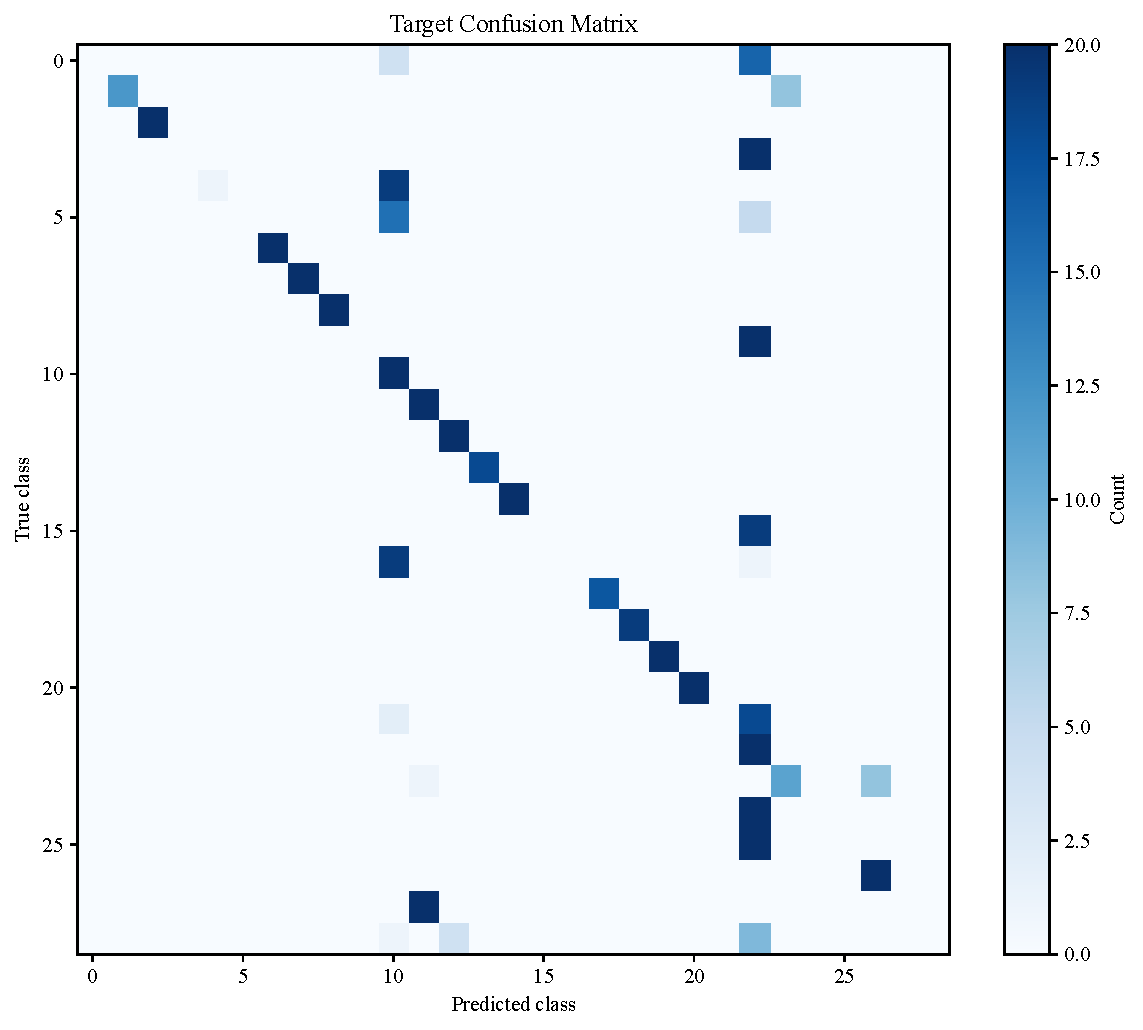
\includegraphics[width=\linewidth,height=0.58\textheight,keepaspectratio]{ch6_single_sourceonly_5_to_2_confusion.pdf}\\[-0.05cm]
      \centering{\small SourceOnly\\\textbf{56.08\%}}
    \end{column}
    \begin{column}{0.31\textwidth}
      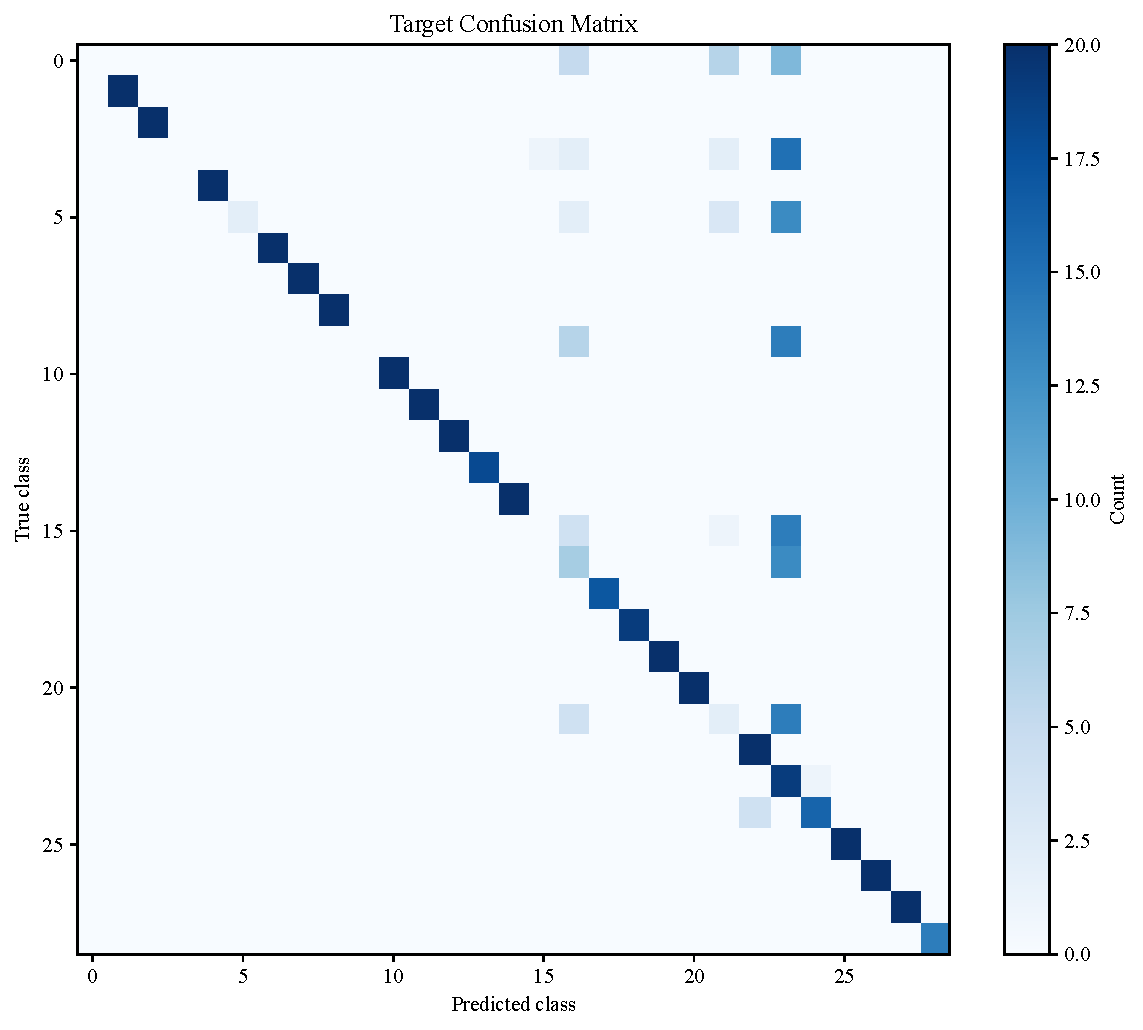
\includegraphics[width=\linewidth,height=0.58\textheight,keepaspectratio]{ch6_single_deepjdot_5_to_2_confusion.pdf}\\[-0.05cm]
      \centering{\small DeepJDOT\\\textbf{67.20\%}}
    \end{column}
    \begin{column}{0.31\textwidth}
      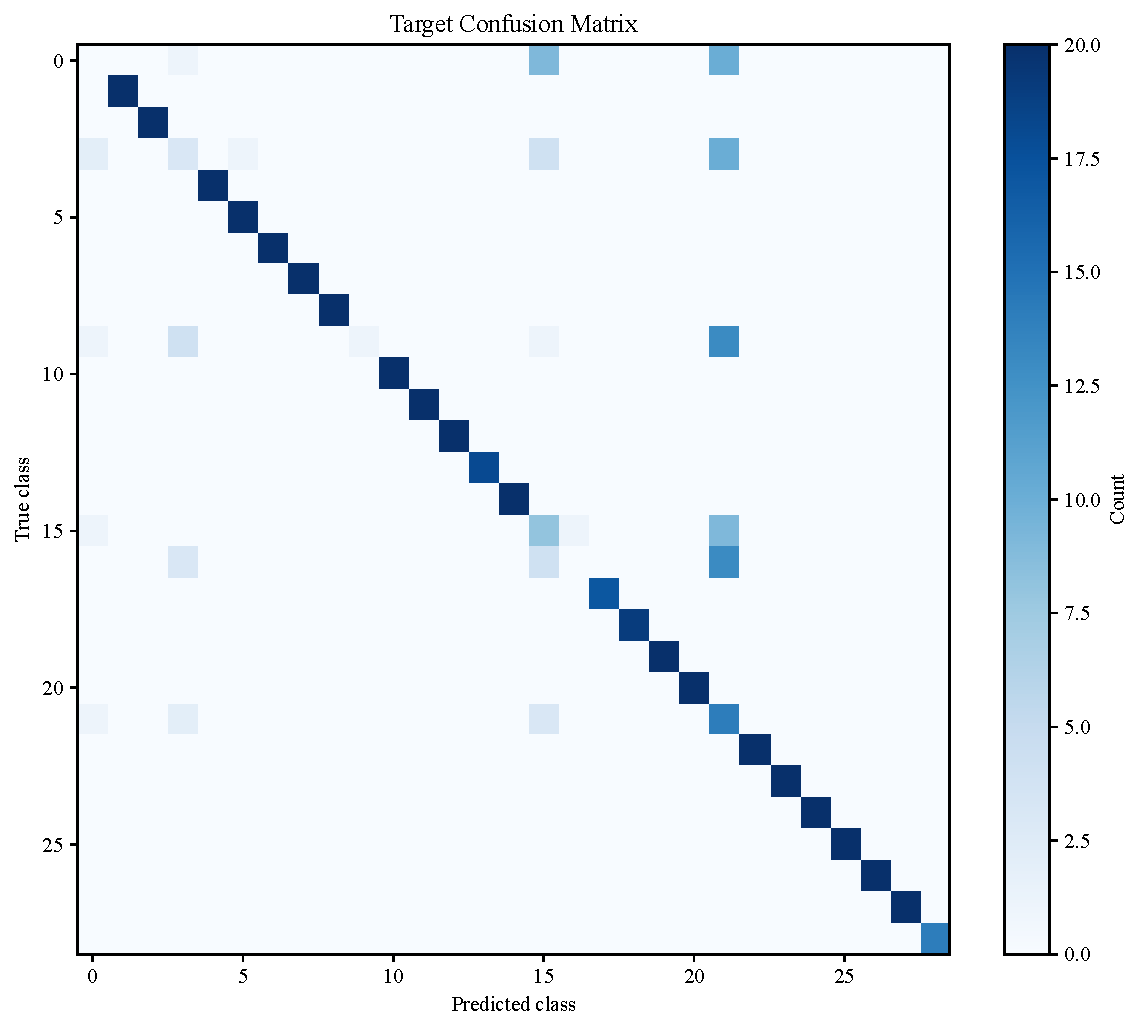
\includegraphics[width=\linewidth,height=0.58\textheight,keepaspectratio]{ch6_single_TPU_DPJDOT_5_to_2_confusion.pdf}\\[-0.05cm]
      \centering{\small TPU-DeepJDOT\\\textbf{83.60\%}}
    \end{column}
  \end{columns}
  \vspace{0.3cm}
  \centering
  {\small\color{muted}混淆矩阵对角线增强：错误强制匹配被削弱，类别结构更清晰。}
\end{frame}

\paperref{P44--45}
\begin{frame}{方法一验证：域分布与类别结构}
  \begin{columns}[T,totalwidth=\textwidth]
    \begin{column}{0.31\textwidth}
      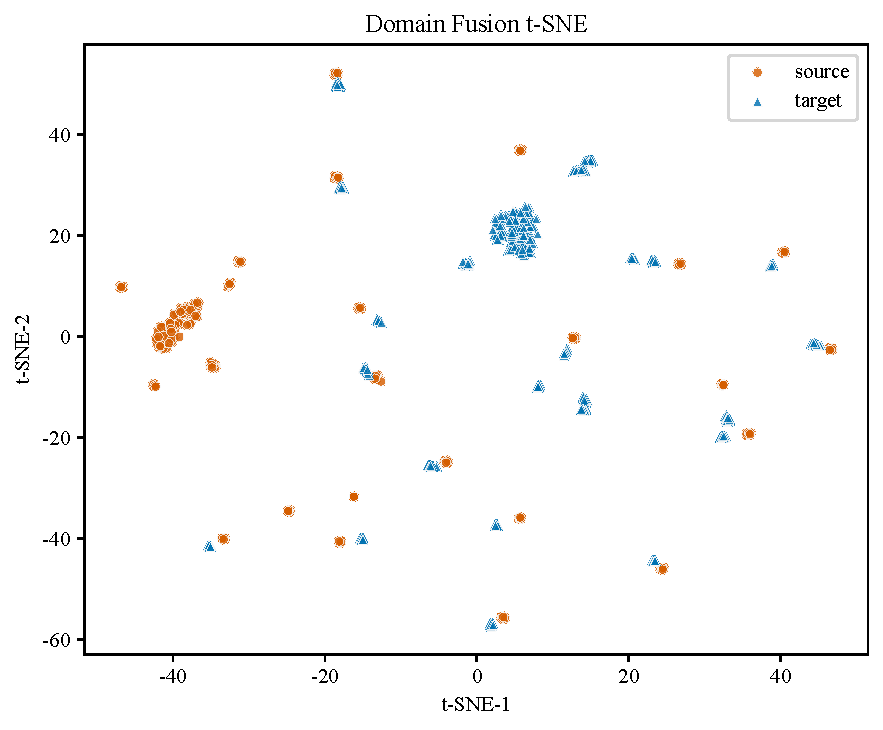
\includegraphics[width=\linewidth,height=0.29\textheight,keepaspectratio]{ch6_single_sourceonly_5_to_2_tsne_domain.pdf}
      \captionline{SourceOnly：域 t-SNE}
      \vspace{0.08cm}
      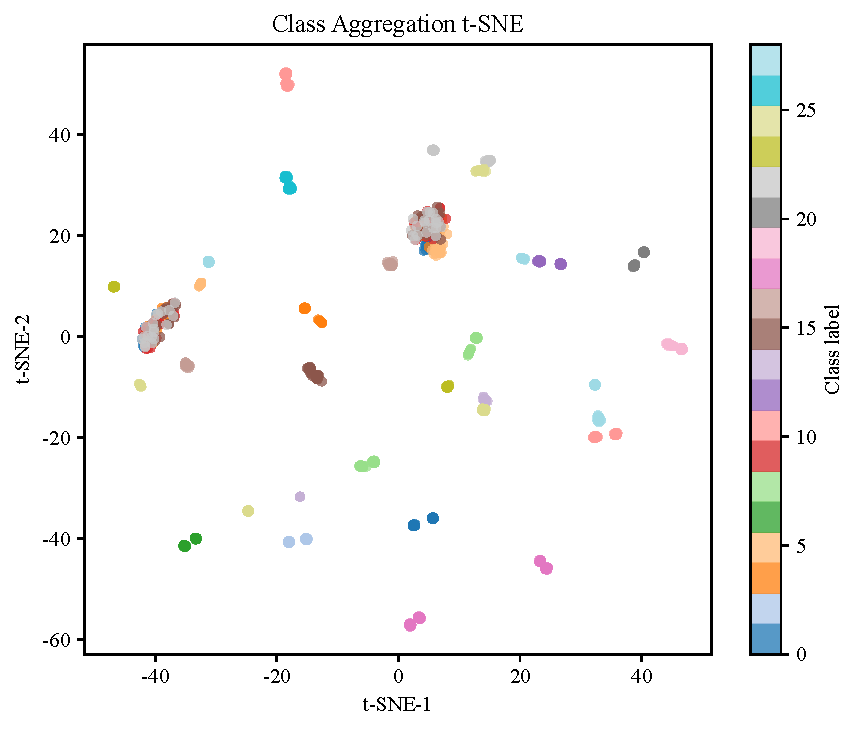
\includegraphics[width=\linewidth,height=0.29\textheight,keepaspectratio]{ch6_single_sourceonly_5_to_2_tsne_class.pdf}
      \captionline{SourceOnly：类 t-SNE}
    \end{column}
    \begin{column}{0.31\textwidth}
      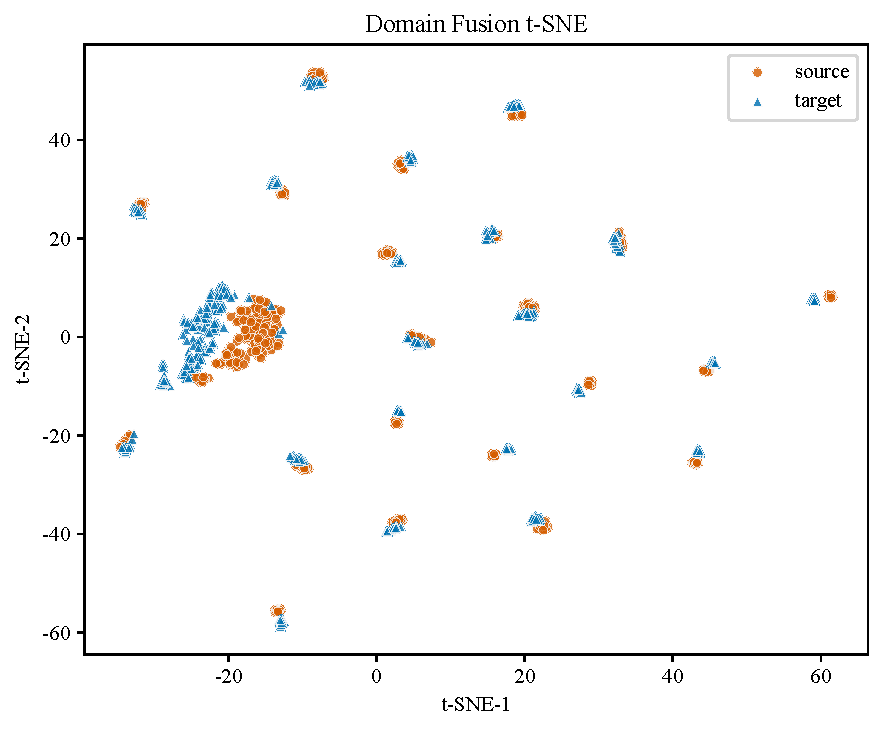
\includegraphics[width=\linewidth,height=0.29\textheight,keepaspectratio]{ch6_single_deepjdot_5_to_2_tsne_domain.pdf}
      \captionline{DeepJDOT：域 t-SNE}
      \vspace{0.08cm}
      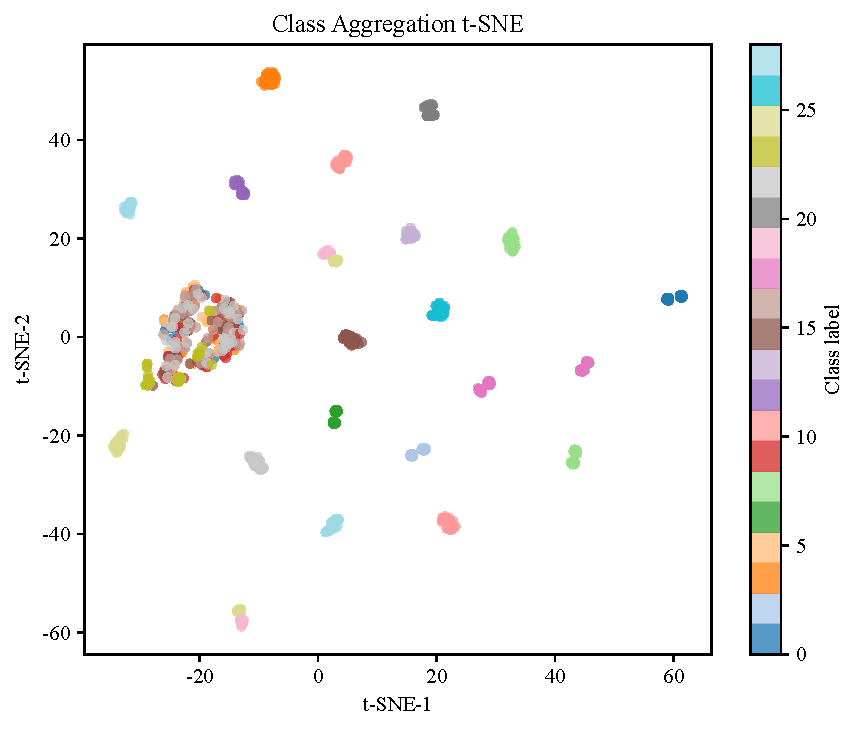
\includegraphics[width=\linewidth,height=0.29\textheight,keepaspectratio]{ch6_single_deepjdot_5_to_2_tsne_class.pdf}
      \captionline{DeepJDOT：类 t-SNE}
    \end{column}
    \begin{column}{0.31\textwidth}
      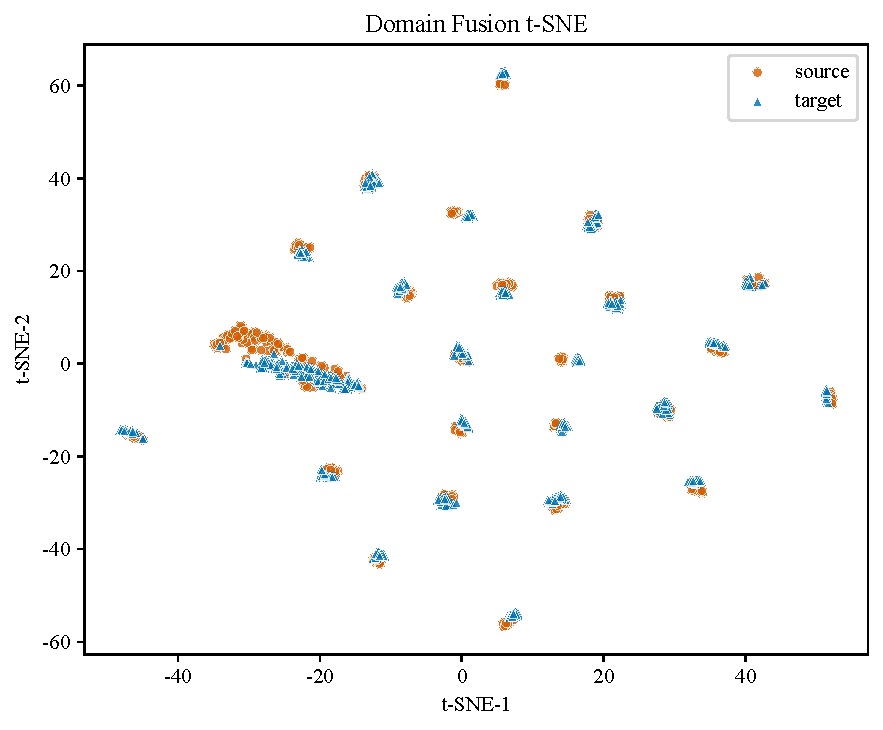
\includegraphics[width=\linewidth,height=0.29\textheight,keepaspectratio]{ch6_single_TPU_DPJDOT_5_to_2_tsne_domain.pdf}
      \captionline{TPU-DeepJDOT：域 t-SNE}
      \vspace{0.08cm}
      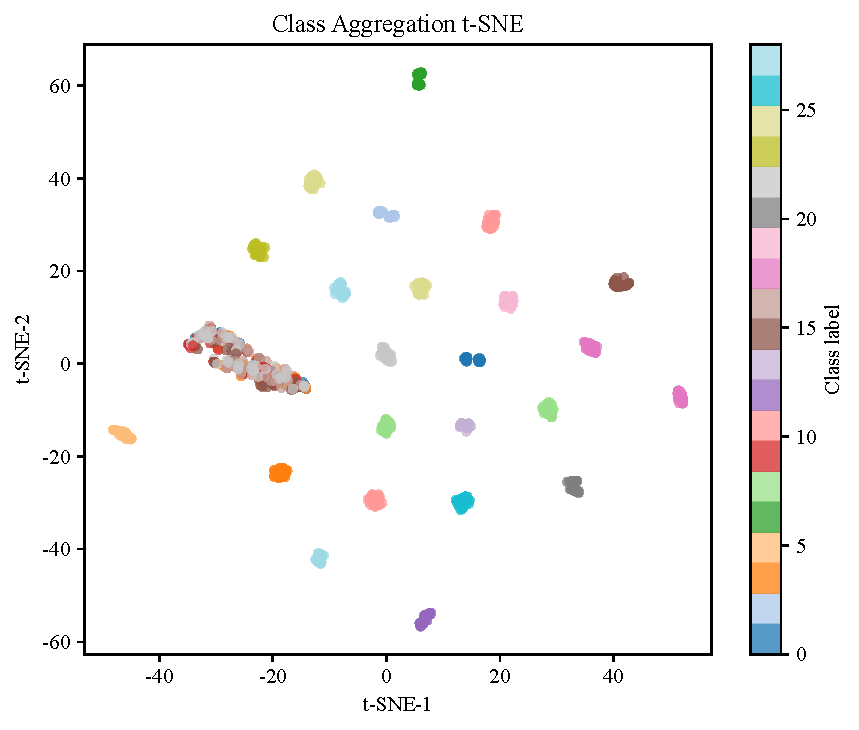
\includegraphics[width=\linewidth,height=0.29\textheight,keepaspectratio]{ch6_single_TPU_DPJDOT_5_to_2_tsne_class.pdf}
      \captionline{TPU-DeepJDOT：类 t-SNE}
    \end{column}
  \end{columns}
\end{frame}

\paperref{P22}
\begin{frame}{方法二：CBTPU-DeepJDOT 架构}
  \centering
  \vspace*{\fill}
  \resizebox{!}{0.86\textheight}{\begin{tikzpicture}[
    x=1cm,
    y=1.35cm,
    >=stealth,
    font=\small\fontspec{Times New Roman}\songti,
    card/.style={draw, rounded corners=4pt, line width=0.45pt, fill=white},
    chip/.style={
        draw,
        rounded corners=2pt,
        line width=0.35pt,
        fill=white,
        align=center,
        inner xsep=5pt,
        inner ysep=5pt
    },
    bluecard/.style={card, draw=blue!45!black, fill=blue!4},
    cyancard/.style={card, draw=cyan!50!black, fill=cyan!5},
    orangecard/.style={card, draw=orange!65!black, fill=orange!6},
    purplecard/.style={card, draw=purple!45!black, fill=purple!5},
    redcard/.style={card, draw=red!45!black, fill=red!5},
    panel/.style={draw=black!15, rounded corners=5pt, line width=0.35pt, fill=gray!1},
    arrow/.style={->, line width=0.55pt, draw=black!70},
    note/.style={font=\scriptsize\fontspec{Times New Roman}\songti, align=center}
]

\draw[panel] (-0.25,0.00) rectangle (21.25,9.00);
\node[font=\large\fontspec{Times New Roman}\songti] at (10.50,8.55)
    {CBTPU-DeepJDOT 多证据置信均衡伪标签控制机制};

% 基础输入
\draw[bluecard] (0.45,2.15) rectangle (3.25,7.75);
\node at (1.85,7.43) {基础信息};
\node[chip, minimum width=2.20cm] at (1.85,6.05)
    {TPU-DeepJDOT\\[-1pt]$\gamma^\ast,\mu_c$};
\node[chip, minimum width=2.20cm] at (1.85,4.60)
    {目标域样本\\[-1pt]$x_j^t$};
\node[note, text width=2.30cm] at (1.85,3.25)
    {继承第三章传输与原型结构};

% 教师-学生增强
\draw[cyancard] (3.95,2.15) rectangle (7.35,7.75);
\node at (5.65,7.43) {教师--学生增强};
\node[chip, minimum width=2.65cm] at (5.65,6.15)
    {弱增强 + 教师锚点\\[-1pt]$a_w(x_j^t),\bar{\Theta}$};
\node[chip, minimum width=2.65cm] at (5.65,4.60)
    {强增强 + 学生\\[-1pt]$a_s(x_j^t),\Theta$};
\node[note, text width=2.70cm] at (5.65,3.25)
    {加载 TPU 检查点；冻结时不参与 EMA};

% 三路证据
\draw[orangecard] (8.05,2.15) rectangle (11.15,7.75);
\node at (9.60,7.43) {三路语义证据};
\node[chip, minimum width=2.35cm] at (9.60,6.20)
    {传输语义\\[-1pt]$q^{ot}$};
\node[chip, minimum width=2.35cm] at (9.60,4.95)
    {教师语义\\[-1pt]$q^{cls}$};
\node[chip, minimum width=2.35cm] at (9.60,3.70)
    {原型语义\\[-1pt]$q^{proto}$};

% 接收门控
\draw[purplecard] (11.85,2.15) rectangle (15.45,7.75);
\node at (13.65,7.43) {可靠接收门控};
\node[chip, minimum width=2.75cm] at (13.65,6.20)
    {多证据融合\\[-1pt]$q^{mix}$};
\node[chip, minimum width=2.75cm, text width=2.65cm] at (13.65,4.90)
    {接收集合 $\mathcal{A}$\\[-1pt]一致 / JS / $\vartheta(\nu)$ / 熵};
\node[chip, minimum width=2.75cm] at (13.65,3.55)
    {接收比例上限\\[-1pt]$\kappa,\,H(q^{ot})$};
\node[note, text width=2.90cm] at (13.65,2.60)
    {只让高可靠目标样本进入伪监督};

% 均衡目标学习
\draw[redcard] (16.15,2.15) rectangle (20.85,7.75);
\node at (18.50,7.43) {均衡目标学习};
\node[chip, minimum width=3.65cm] at (18.50,6.20)
    {类别均衡伪监督\\[-1pt]$\mathcal{L}_{pl},\ \hat{\pi}_c$};
\node[chip, minimum width=3.65cm] at (18.50,4.95)
    {强弱增强一致性\\[-1pt]$\mathcal{L}_{cons}$};
\node[chip, minimum width=3.65cm] at (18.50,3.70)
    {信息最大化辅助\\[-1pt]$\mathcal{L}_{im}$};
\node[note, text width=3.75cm] at (18.50,2.60)
    {降低伪标签噪声与类别坍缩};

% 目标域学习
\draw[redcard] (3.95,0.50) rectangle (20.85,1.35);
\node at (12.40,0.92)
    {$\mathcal{L}_{CBTPU}
    =\mathcal{L}_{TPU}
    +\lambda_{pl}\mathcal{L}_{pl}
    +\lambda_{cons}\mathcal{L}_{cons}
    +\lambda_{im}\mathcal{L}_{im}$};

\draw[arrow] (3.25,4.95) -- (3.95,4.95);
\draw[arrow] (7.35,4.95) -- (8.05,4.95);
\draw[arrow] (11.15,4.95) -- (11.85,4.95);
\draw[arrow] (15.45,4.95) -- (16.15,4.95);
\draw[arrow] (18.50,2.15) -- (18.50,1.35);

\end{tikzpicture}
}
  \vspace*{\fill}
\end{frame}

\paperref{P25}
\begin{frame}{方法二：多证据伪标签筛选}
  \vspace*{0.32cm}
  \formularow{blue!4}{证据融合}{
    q_{jc}^{\mathrm{mix}}=
    \frac{(q_{jc}^{\mathrm{ot}})^{\alpha_{\mathrm{ot}}}
    (q_{jc}^{\mathrm{cls}})^{\alpha_{\mathrm{cls}}}
    (q_{jc}^{\mathrm{proto}})^{\alpha_{\mathrm{proto}}}}
    {\sum_{c'=1}^{N_c}(q_{jc'}^{\mathrm{ot}})^{\alpha_{\mathrm{ot}}}
    (q_{jc'}^{\mathrm{cls}})^{\alpha_{\mathrm{cls}}}
    (q_{jc'}^{\mathrm{proto}})^{\alpha_{\mathrm{proto}}}}
  }{4-12}
  \formulagap
  \formularow{green!5}{接收条件}{
    \mathcal{A}_j=[\hat y_j^{\mathrm{ot}}=\hat y_j^{\mathrm{cls}}=\hat y_j^{\mathrm{proto}}\ \mathrm{or}\ D_{\mathrm{JS}}\leq\delta_{\mathrm{JS}}]
    \land[\max_c q_{jc}^{\mathrm{mix}}\geq\vartheta(\nu)]
    \land[H(q_j^{\mathrm{ot}})\leq h_{\mathrm{ot}}]
  }{4-15}
  \formulagap
  \formularow{amber!5}{总目标}{
    \mathcal{L}_{\mathrm{CBTPU}}=\mathcal{L}_{\mathrm{src}}
    +\lambda_{\mathrm{supcon}}(\nu)\mathcal{L}_{\mathrm{supcon}}
    +\lambda_{\mathrm{ot}}(\nu)\mathcal{L}_{\mathrm{align}}
    +\lambda_{\mathrm{pl}}(\nu)\mathcal{L}_{\mathrm{pl}}
    +\lambda_{\mathrm{cons}}(\nu)\mathcal{L}_{\mathrm{cons}}
    +\lambda_{\mathrm{im}}(\nu)\mathcal{L}_{\mathrm{im}}
  }{4-22}
\end{frame}

\paperref{P28}
\begin{frame}{方法二：CBTPU-DeepJDOT 训练流程}
  \begin{columns}[c,onlytextwidth,totalwidth=\textwidth]
    \begin{column}{0.58\textwidth}
      \centering
      \resizebox{\linewidth}{!}{%
      \begin{tikzpicture}[node distance=0.40cm]
        \node[box, fill=blue!7, draw=blue!35, minimum width=2.62cm] (a) {初始化学生/教师\\继承 TPU};
        \node[box, fill=teal!7, draw=teal!35, minimum width=2.62cm, right=0.42cm of a] (b) {目标弱增强\\目标强增强};
        \node[box, fill=amber!9, draw=amber!40, minimum width=2.62cm, right=0.42cm of b] (c) {三类证据\\传输/教师/原型};
        \node[box, fill=violet!8, draw=violet!40, minimum width=2.62cm, below=0.86cm of c] (d) {融合与筛选\\$\mathcal{A}$};
        \node[box, fill=green!8, draw=green!35, minimum width=2.62cm, left=0.42cm of d] (e) {伪标签学习\\强弱一致性};
        \node[box, fill=red!6, draw=red!35, minimum width=2.62cm, left=0.42cm of e] (f) {更新学生\\维护教师};
        \draw[arrow] (a) -- (b);
        \draw[arrow] (b) -- (c);
        \draw[arrow] (c) -- (d);
        \draw[arrow] (d) -- (e);
        \draw[arrow] (e) -- (f);
      \end{tikzpicture}
      }
    \end{column}
    \begin{column}{0.37\textwidth}
      \centering
      \resizebox{\linewidth}{!}{%
      \begin{tikzpicture}[
        flow/.style={box, minimum width=2.32cm, minimum height=0.62cm, inner xsep=5pt, inner ysep=4pt},
        core/.style={box, minimum width=2.48cm, minimum height=0.78cm, inner xsep=6pt, inner ysep=5pt},
        result/.style={box, minimum width=2.54cm, minimum height=0.78cm, inner xsep=6pt, inner ysep=5pt}
      ]
        \node[flow, fill=blue!7, draw=blue!35] (ot) at (0,1.50) {传输语义\\$q^{\mathrm{ot}}$};
        \node[flow, fill=teal!7, draw=teal!35] (tea) at (0,0.30) {固定教师\\预测 $q^{\mathrm{cls}}$};
        \node[flow, fill=amber!9, draw=amber!40] (pro) at (0,-0.90) {源域原型\\$q^{\mathrm{proto}}$};
        \node[core, fill=green!8, draw=green!35] (mix) at (2.96,0.36) {幂加权融合\\$q^{\mathrm{mix}}$};
        \node[result, fill=red!6, draw=red!35] (gate) at (2.96,-1.28) {一致性 + 置信度\\+ 传输熵门控};
        \draw[thinarr] (ot.east) -- ([yshift=0.24cm]mix.west);
        \draw[thinarr] (tea.east) -- (mix.west);
        \draw[thinarr] (pro.east) -- ([yshift=-0.24cm]mix.west);
        \draw[arrow] (mix.south) -- (gate.north);
      \end{tikzpicture}
      }
    \end{column}
  \end{columns}
\end{frame}

\paperref{P46}
\begin{frame}{方法二验证：$m_5\rightarrow m_1$ 伪标签细化}
  \begin{columns}[T,totalwidth=\textwidth]
    \begin{column}{0.38\textwidth}
      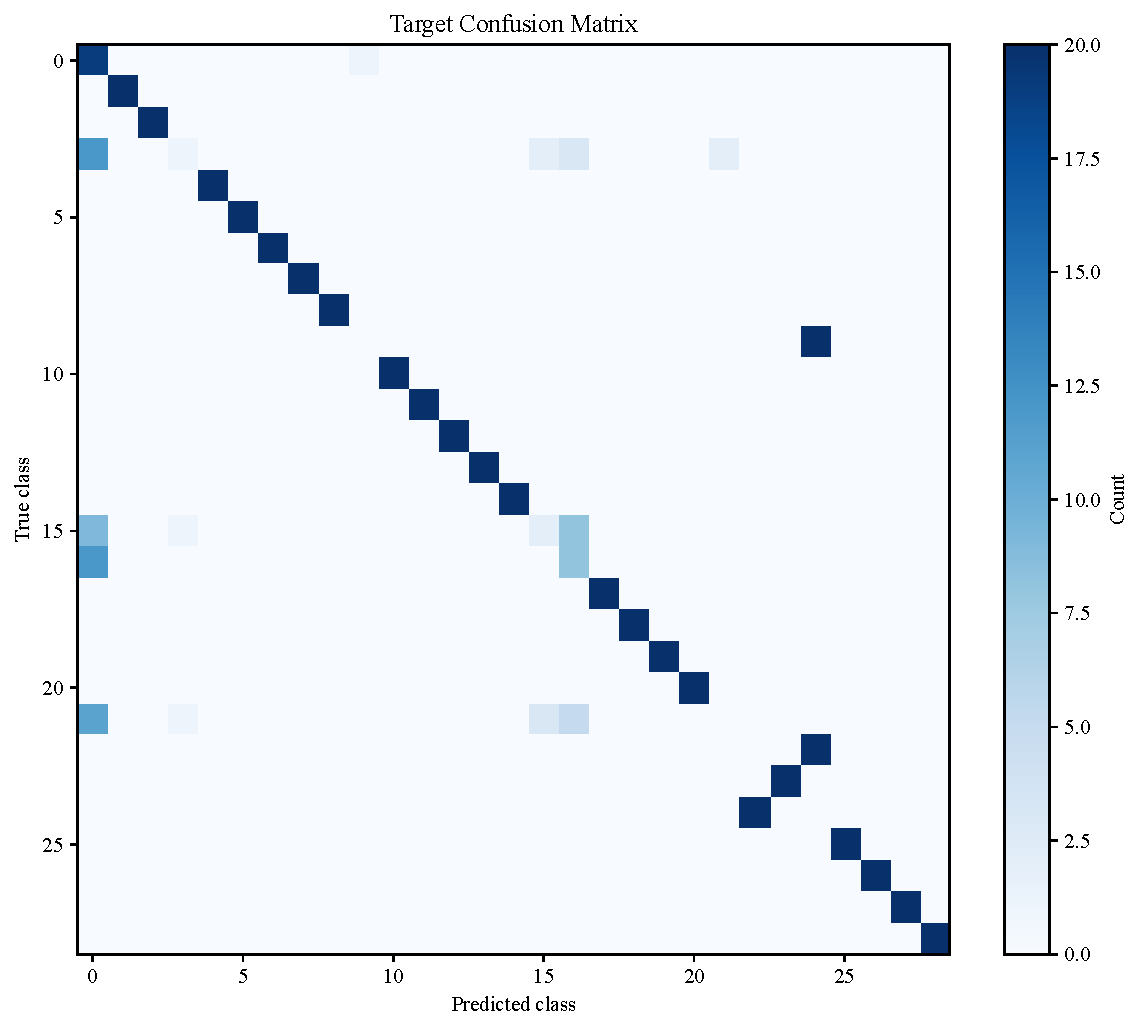
\includegraphics[width=\linewidth,height=0.62\textheight,keepaspectratio]{ch6_single_TPU_DPJDOT_5_to_1_confusion.pdf}\\[-0.05cm]
      \centering{\small TPU-DeepJDOT\\\textbf{77.59\%}}
    \end{column}
    \begin{column}{0.38\textwidth}
      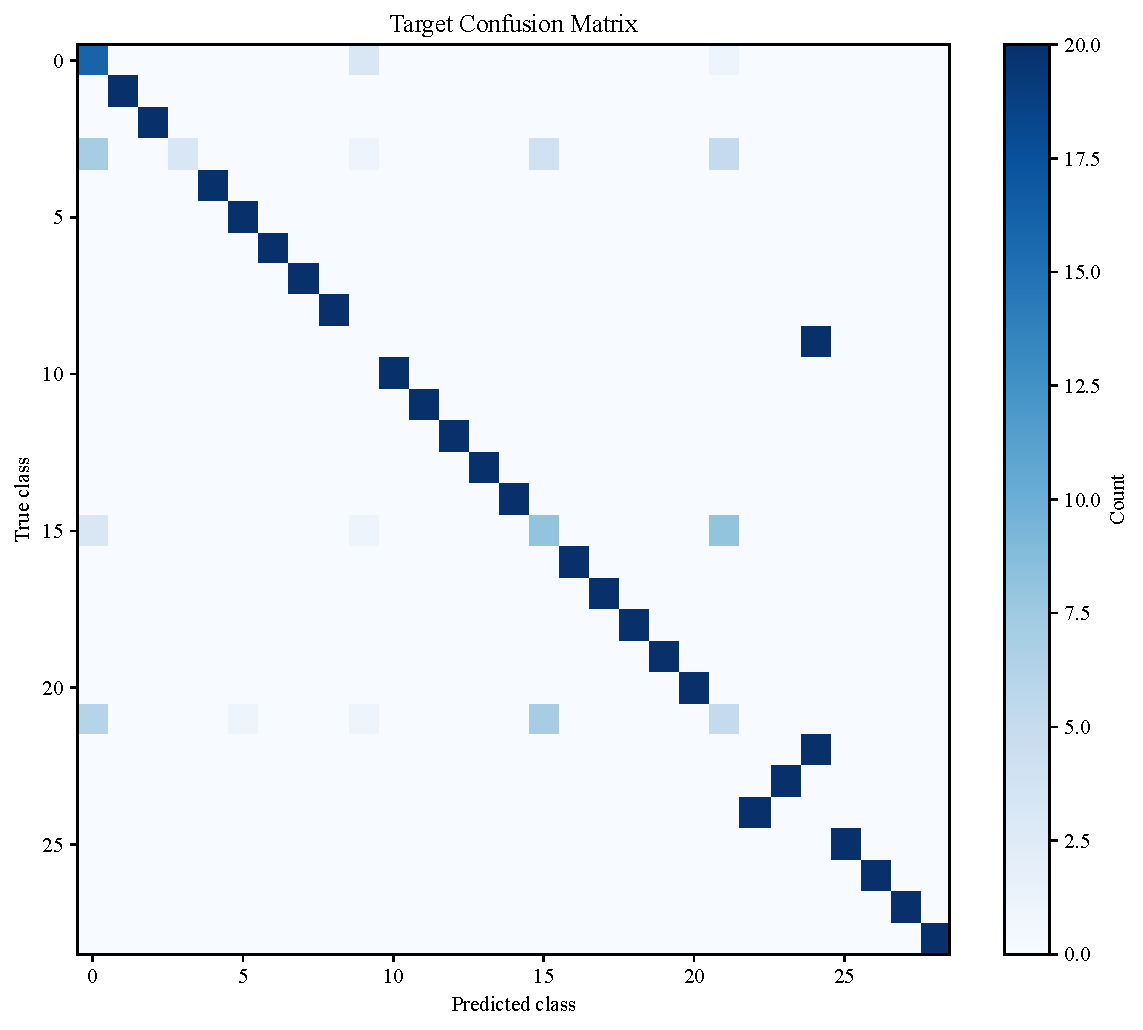
\includegraphics[width=\linewidth,height=0.62\textheight,keepaspectratio]{ch6_single_CBTPU_DPJDOT_5_to_1_confusion.pdf}\\[-0.05cm]
      \centering{\small CBTPU-DeepJDOT\\\textbf{81.38\%}}
    \end{column}
    \begin{column}{0.20\textwidth}
      \vspace{0.55cm}
      \tagpill{teal}{三证据筛选}\\[0.16cm]
      \tagpill{amber}{类别均衡}\\[0.16cm]
      \tagpill{violet}{强弱一致性}\\[0.45cm]
      {\small\color{muted}不是追求伪标签数量，而是控制进入训练的噪声。}
    \end{column}
  \end{columns}
\end{frame}

\paperref{P46--47}
\begin{frame}{方法二验证：局部边界继续收紧}
  \begin{columns}[T,totalwidth=\textwidth]
    \begin{column}{0.48\textwidth}
      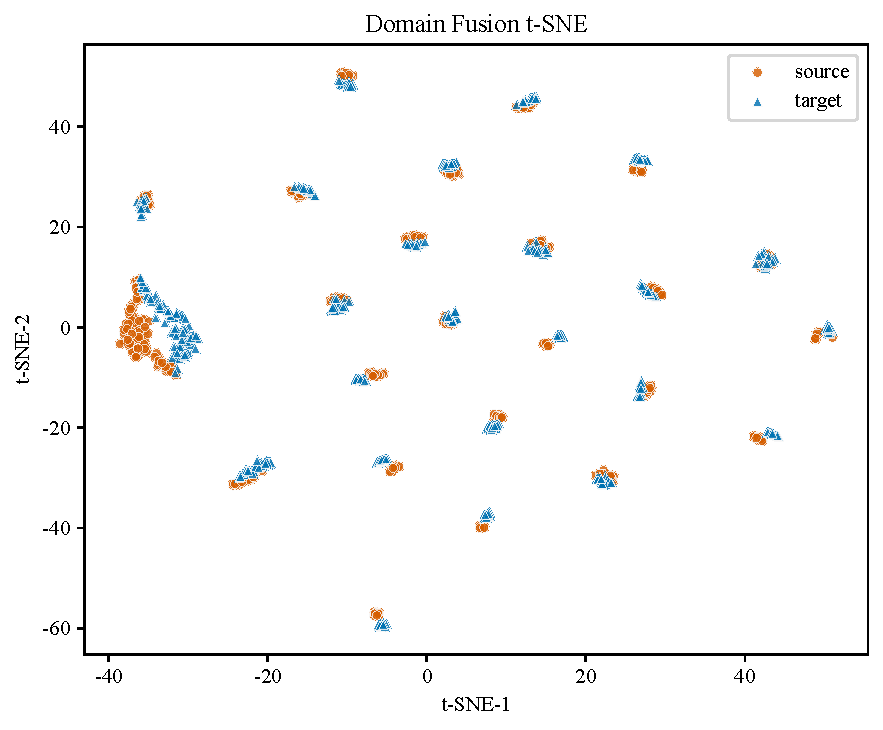
\includegraphics[width=\linewidth,height=0.31\textheight,keepaspectratio]{ch6_single_TPU_DPJDOT_5_to_1_tsne_domain.pdf}
      \captionline{TPU-DeepJDOT：域 t-SNE}
      \vspace{0.08cm}
      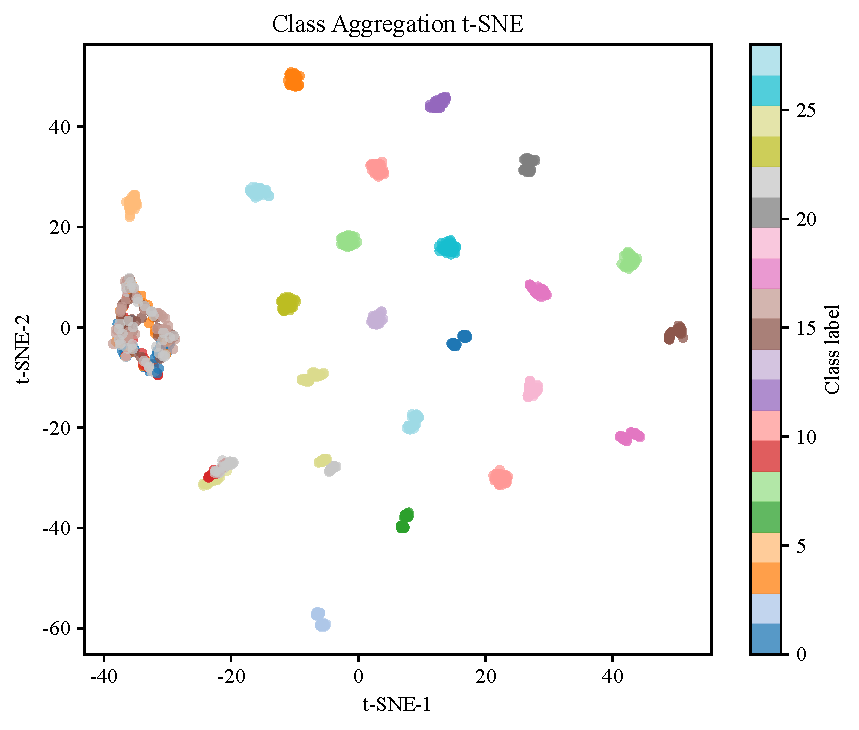
\includegraphics[width=\linewidth,height=0.31\textheight,keepaspectratio]{ch6_single_TPU_DPJDOT_5_to_1_tsne_class.pdf}
      \captionline{TPU-DeepJDOT：类 t-SNE}
    \end{column}
    \begin{column}{0.48\textwidth}
      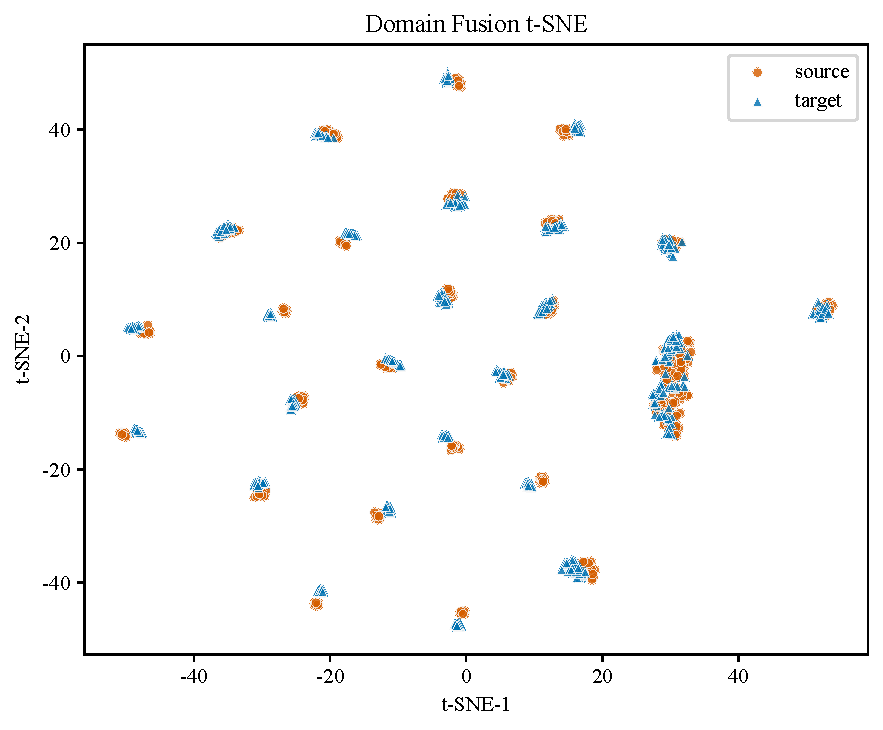
\includegraphics[width=\linewidth,height=0.31\textheight,keepaspectratio]{ch6_single_CBTPU_DPJDOT_5_to_1_tsne_domain.pdf}
      \captionline{CBTPU-DeepJDOT：域 t-SNE}
      \vspace{0.08cm}
      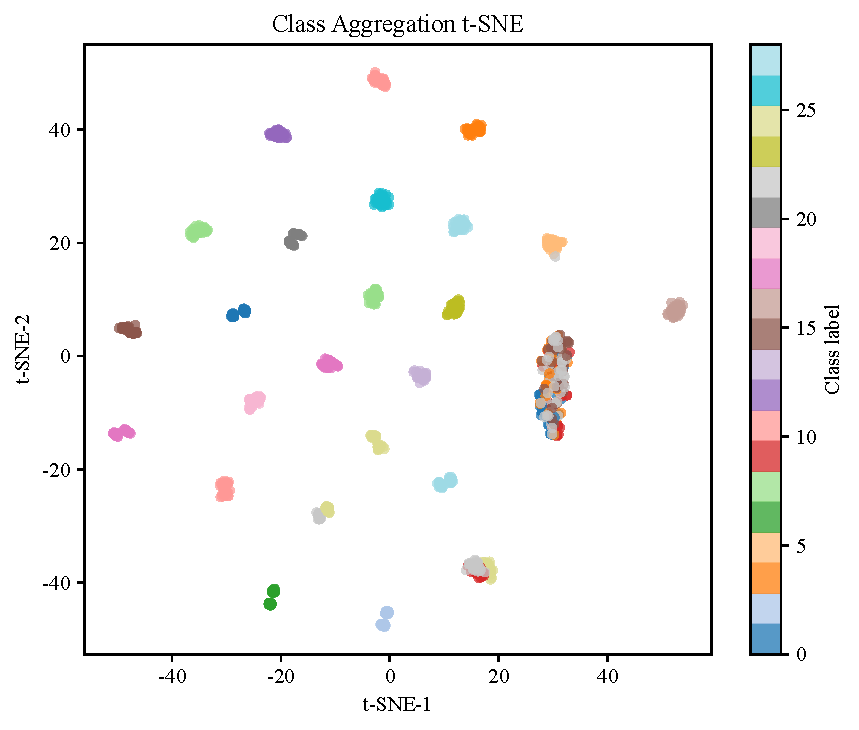
\includegraphics[width=\linewidth,height=0.31\textheight,keepaspectratio]{ch6_single_CBTPU_DPJDOT_5_to_1_tsne_class.pdf}
      \captionline{CBTPU-DeepJDOT：类 t-SNE}
    \end{column}
  \end{columns}
\end{frame}

\paperref{P30}
\begin{frame}{方法三：CA-CCSR-WJDOT 架构}
  \centering
  \vspace*{\fill}
  \resizebox{!}{0.86\textheight}{\begin{tikzpicture}[
    x=1cm,
    y=1.35cm,
    >=stealth,
    font=\small\fontspec{Times New Roman}\songti,
    card/.style={draw, rounded corners=4pt, line width=0.45pt, fill=white},
    chip/.style={
        draw,
        rounded corners=2pt,
        line width=0.35pt,
        fill=white,
        align=center,
        inner xsep=5pt,
        inner ysep=4pt
    },
    bluecard/.style={card, draw=blue!45!black, fill=blue!4},
    cyancard/.style={card, draw=cyan!50!black, fill=cyan!5},
    greencard/.style={card, draw=green!45!black, fill=green!6},
    orangecard/.style={card, draw=orange!65!black, fill=orange!6},
    purplecard/.style={card, draw=purple!45!black, fill=purple!5},
    redcard/.style={card, draw=red!45!black, fill=red!5},
    panel/.style={draw=black!15, rounded corners=5pt, line width=0.35pt, fill=gray!1},
    arrow/.style={->, line width=0.55pt, draw=black!70},
    note/.style={font=\scriptsize\fontspec{Times New Roman}\songti, align=center}
]

\draw[panel] (-0.25,0.00) rectangle (21.25,9.00);
\node[font=\large\fontspec{Times New Roman}\songti] at (10.50,8.55)
    {CA-CCSR-WJDOT 类条件源域可靠性加权机制};

\begin{scope}[xshift=-0.15cm]

% 多源输入
\draw[bluecard] (0.45,2.15) rectangle (3.05,7.75);
\node at (1.75,7.43) {多源输入};
\node[chip, minimum width=1.95cm] at (1.75,6.35) {源域 $s_1$};
\node[chip, minimum width=1.95cm] at (1.75,5.35) {源域 $s_2$};
\node[chip, minimum width=1.95cm] at (1.75,4.35) {源域 $s_K$};
\node[chip, minimum width=1.95cm] at (1.75,3.35) {目标域 $\mathcal{D}_t$};
\node[note, text width=2.15cm] at (1.75,2.55)
    {源域身份保留到逐源传输};

% CoDATS 表征与教师
\draw[cyancard] (3.75,2.15) rectangle (7.35,7.75);
\node at (5.55,7.43) {CoDATS 表征};
\node[chip, minimum width=2.80cm] at (5.55,6.20)
    {共享 FCN + 分类头\\[-1pt]$F_\theta,\ G_\phi$};
\node[chip, minimum width=2.80cm] at (5.55,4.95)
    {领域对抗约束\\[-1pt]$\mathcal{L}_{\mathrm{dom}}$};
\node[chip, minimum width=2.80cm] at (5.55,3.70)
    {教师先验保护\\[-1pt]$\bar{\Theta}_{C},\ \mathcal{L}_{\mathrm{tea}}$};
\node[note, text width=2.90cm] at (5.55,2.60)
    {提供稳定跨域时序表征};

% 逐源传输
\draw[greencard] (8.05,2.15) rectangle (11.65,7.75);
\node at (9.85,7.43) {逐源联合传输};
\node[chip, minimum width=2.80cm] at (9.85,6.20)
    {$s_k\rightarrow t$ 独立传输\\[-1pt]$\gamma_k^\ast$};
\node[chip, minimum width=2.80cm] at (9.85,4.95)
    {类条件统计\\[-1pt]$D_{kc}^{\mathrm{ot}},\ M_{kc}^{\mathrm{ot}}$};
\node[chip, minimum width=2.80cm] at (9.85,3.70)
    {逐源聚合\\[-1pt]$\mathcal{L}_{\mathrm{WJDOT}}$};
\node[note, text width=2.90cm] at (9.85,2.60)
    {不再简单合并多源批次};

% 可靠性矩阵
\draw[orangecard] (12.35,2.15) rectangle (15.95,7.75);
\node at (14.15,7.43) {可靠性证据};
\node[chip, minimum width=2.80cm] at (14.15,6.20)
    {原型距离\\[-1pt]$D_{kc}^{\mathrm{proto}}$};
\node[chip, minimum width=2.80cm] at (14.15,4.95)
    {传输与熵\\[-1pt]$D_{kc}^{\mathrm{ot}},\ H_{kc}^{\mathrm{pred}}$};
\node[chip, minimum width=2.80cm] at (14.15,3.70)
    {源类性能\\[-1pt]$E_{kc}^{s}$};
\node[note, text width=2.90cm] at (14.15,2.60)
    {归一组合为可靠性矩阵 $R_{kc}$};

% 类条件权重与融合
\draw[purplecard] (16.65,2.15) rectangle (20.85,7.75);
\node at (18.75,7.43) {类条件权重与融合};
\node[chip, minimum width=3.20cm] at (18.75,6.35)
    {可靠性到权重\\[-1pt]$R_{kc}\rightarrow\alpha_{kc}$};
\node[chip, minimum width=3.20cm] at (18.75,5.20)
    {类条件传输损失\\[-1pt]$\mathcal{L}_{\mathrm{CCSR}}$};
\node[chip, minimum width=3.20cm] at (18.75,4.05)
    {教师先验融合\\[-1pt]$p^{\mathrm{final}}$};
\begin{scope}[shift={(17.72,2.50)}]
    \node[font=\tiny\fontspec{Times New Roman}\songti] at (-0.34,0.56)
        {源域};
    \node[font=\tiny\fontspec{Times New Roman}\songti] at (0.84,0.74)
        {故障类别};
    \node[font=\tiny\fontspec{Times New Roman}\songti] at (2.33,0.74)
        {迁移可靠性};
    \node[font=\tiny\fontspec{Times New Roman}] at (0.14,0.56) {$c_1$};
    \node[font=\tiny\fontspec{Times New Roman}] at (0.42,0.56) {$c_2$};
    \node[font=\tiny\fontspec{Times New Roman}] at (0.98,0.56) {$\cdots$};
    \node[font=\tiny\fontspec{Times New Roman}] at (1.54,0.56) {$c_{N_c}$};
    \node[font=\tiny\fontspec{Times New Roman}, anchor=east] at (-0.12,0.40) {$s_1$};
    \node[font=\tiny\fontspec{Times New Roman}, anchor=east] at (-0.12,0.24) {$s_2$};
    \node[font=\tiny\fontspec{Times New Roman}, anchor=east] at (-0.12,0.08) {$s_K$};
    \draw[draw=black!35, line width=0.20pt, fill=green!35] (0.00,0.32) rectangle (0.28,0.48);
    \draw[draw=black!35, line width=0.20pt, fill=green!15] (0.28,0.32) rectangle (0.56,0.48);
    \draw[draw=black!35, line width=0.20pt, fill=yellow!18] (0.56,0.32) rectangle (0.84,0.48);
    \draw[draw=black!35, line width=0.20pt, fill=green!25] (0.84,0.32) rectangle (1.12,0.48);
    \draw[draw=black!35, line width=0.20pt, fill=yellow!22] (1.12,0.32) rectangle (1.40,0.48);
    \draw[draw=black!35, line width=0.20pt, fill=green!45] (1.40,0.32) rectangle (1.68,0.48);
    \draw[draw=black!35, line width=0.20pt, fill=yellow!28] (0.00,0.16) rectangle (0.28,0.32);
    \draw[draw=black!35, line width=0.20pt, fill=green!42] (0.28,0.16) rectangle (0.56,0.32);
    \draw[draw=black!35, line width=0.20pt, fill=green!18] (0.56,0.16) rectangle (0.84,0.32);
    \draw[draw=black!35, line width=0.20pt, fill=yellow!16] (0.84,0.16) rectangle (1.12,0.32);
    \draw[draw=black!35, line width=0.20pt, fill=green!30] (1.12,0.16) rectangle (1.40,0.32);
    \draw[draw=black!35, line width=0.20pt, fill=yellow!26] (1.40,0.16) rectangle (1.68,0.32);
    \draw[draw=black!35, line width=0.20pt, fill=green!18] (0.00,0.00) rectangle (0.28,0.16);
    \draw[draw=black!35, line width=0.20pt, fill=yellow!24] (0.28,0.00) rectangle (0.56,0.16);
    \draw[draw=black!35, line width=0.20pt, fill=green!38] (0.56,0.00) rectangle (0.84,0.16);
    \draw[draw=black!35, line width=0.20pt, fill=green!12] (0.84,0.00) rectangle (1.12,0.16);
    \draw[draw=black!35, line width=0.20pt, fill=green!46] (1.12,0.00) rectangle (1.40,0.16);
    \draw[draw=black!35, line width=0.20pt, fill=yellow!18] (1.40,0.00) rectangle (1.68,0.16);
    \shade[bottom color=yellow!12, top color=green!55, draw=black!35, line width=0.20pt]
        (2.05,0.00) rectangle (2.19,0.48);
    \node[font=\tiny\fontspec{Times New Roman}\songti, anchor=west] at (2.27,0.48) {高};
    \node[font=\tiny\fontspec{Times New Roman}\songti, anchor=west] at (2.27,0.00) {低};
\end{scope}

% 总目标
\draw[redcard] (0.45,0.50) rectangle (20.85,1.35);
\node[align=center] at (10.65,0.92)
    {$\mathcal{L}_{\mathrm{CA}\text{-}\mathrm{CCSR}}
    =\lambda_s\mathcal{L}_{\mathrm{src}}
    +\lambda_d\mathcal{L}_{\mathrm{dom}}
    +\lambda_{\mathrm{ot}}\mathcal{L}_{\mathrm{WJDOT}}
    +\lambda_{\mathrm{ccsr}}\mathcal{L}_{\mathrm{CCSR}}
    +\lambda_{\mathrm{tea}}\mathcal{L}_{\mathrm{tea}}$};

\draw[arrow] (3.05,4.95) -- (3.75,4.95);
\draw[arrow] (7.35,4.95) -- (8.05,4.95);
\draw[arrow] (11.65,4.95) -- (12.35,4.95);
\draw[arrow] (15.95,4.95) -- (16.65,4.95);
\draw[arrow] (18.75,2.15) -- (18.75,1.35);

\end{scope}

\end{tikzpicture}
}
  \vspace*{\fill}
\end{frame}

\paperref{P33}
\begin{frame}{方法三：类条件源域可靠性}
  \vspace*{0.22cm}
  \formularow{blue!4}{可靠性评分}{
    R_{kc}=w_p\widetilde{D}_{kc}^{\mathrm{proto}}
    +w_o\widetilde{D}_{kc}^{\mathrm{ot}}
    +w_h\widetilde{H}_{kc}^{\mathrm{pred}}
    +w_e\widetilde{E}_{kc}^{s}
  }{5-14}
  \formulagap
  \formularow{green!5}{源域权重}{
    \alpha_{kc}=\frac{\exp(-R_{kc}/T_{\mathrm{rel}})}
    {\sum_{k'=1}^{K}\exp(-R_{k'c}/T_{\mathrm{rel}})}
  }{5-15}
  \formulagap
  \formularow{violet!5}{CCSR约束}{
    \mathcal{L}_{\mathrm{CCSR}}=
    \frac{1}{|\mathcal{C}_{\mathrm{act}}|}
    \sum_{c\in\mathcal{C}_{\mathrm{act}}}\sum_{k=1}^{K}
    \mathbb{I}_{kc}\alpha_{kc}D_{kc}^{\mathrm{ot}}
  }{5-17}
  \formulagap
  \formularow{amber!5}{总目标}{
    \mathcal{L}_{\mathrm{CA}\text{-}\mathrm{CCSR}}
    =\lambda_s\mathcal{L}_{\mathrm{src}}
    +\lambda_d(\nu)\mathcal{L}_{\mathrm{dom}}
    +\lambda_{\mathrm{ot}}r_{\mathrm{ot}}(\nu)\mathcal{L}_{\mathrm{WJDOT}}
    +\lambda_{\mathrm{ccsr}}r_{\mathrm{ccsr}}(\nu)\mathcal{L}_{\mathrm{CCSR}}
    +\lambda_{\mathrm{tea}}(\nu)\mathcal{L}_{\mathrm{tea}}
  }{5-22}
\end{frame}

\paperref{P36}
\begin{frame}{方法三：CA-CCSR-WJDOT 训练流程}
  \begin{columns}[c,onlytextwidth,totalwidth=\textwidth]
    \begin{column}{0.58\textwidth}
      \centering
      \resizebox{\linewidth}{!}{%
      \begin{tikzpicture}[node distance=0.38cm]
        \node[box, fill=blue!7, draw=blue!35, minimum width=2.55cm] (a) {初始化\\FCN/CoDATS/教师};
        \node[box, fill=teal!7, draw=teal!35, minimum width=2.55cm, right=0.42cm of a] (b) {多源采样\\目标无标签};
        \node[box, fill=amber!9, draw=amber!40, minimum width=2.55cm, right=0.42cm of b] (c) {逐源传输\\$\gamma_k^\ast,D_{kc}^{\mathrm{ot}}$};
        \node[box, fill=violet!8, draw=violet!40, minimum width=2.55cm, below=0.86cm of c] (d) {可靠性矩阵\\$R_{kc}\rightarrow\alpha_{kc}$};
        \node[box, fill=green!8, draw=green!35, minimum width=2.55cm, left=0.42cm of d] (e) {CCSR/WJDOT\\对抗/教师先验};
        \node[box, fill=red!6, draw=red!35, minimum width=2.55cm, left=0.42cm of e] (f) {更新模型\\目标预测};
        \draw[arrow] (a) -- (b);
        \draw[arrow] (b) -- (c);
        \draw[arrow] (c) -- (d);
        \draw[arrow] (d) -- (e);
        \draw[arrow] (e) -- (f);
      \end{tikzpicture}
      }
    \end{column}
    \begin{column}{0.37\textwidth}
      \centering
      \resizebox{\linewidth}{!}{%
      \begin{tikzpicture}[
        flow/.style={box, minimum width=2.24cm, minimum height=0.58cm, inner xsep=5pt, inner ysep=4pt},
        core/.style={box, minimum width=2.44cm, minimum height=0.78cm, inner xsep=6pt, inner ysep=5pt},
        result/.style={box, minimum width=2.52cm, minimum height=0.74cm, inner xsep=6pt, inner ysep=5pt}
      ]
        \node[flow, fill=blue!7, draw=blue!35] (a) at (0,2.05) {源目标\\原型距离};
        \node[flow, fill=teal!7, draw=teal!35] (b) at (0,0.86) {类条件\\传输代价};
        \node[flow, fill=amber!9, draw=amber!40] (c) at (0,-0.33) {目标预测\\熵};
        \node[flow, fill=violet!8, draw=violet!40] (d) at (0,-1.52) {源域类别\\召回误差};
        \node[core, fill=green!8, draw=green!35] (r) at (2.94,0.28) {$R_{kc}$\\$\rightarrow\alpha_{kc}$};
        \node[result, fill=red!6, draw=red!35] (l) at (2.94,-1.54) {按类别分配\\源域贡献};
        \draw[thinarr] (a.east) -- ([yshift=0.28cm]r.west);
        \draw[thinarr] (b.east) -- ([yshift=0.09cm]r.west);
        \draw[thinarr] (c.east) -- ([yshift=-0.09cm]r.west);
        \draw[thinarr] (d.east) -- ([yshift=-0.28cm]r.west);
        \draw[arrow] (r.south) -- (l.north);
      \end{tikzpicture}
      }
    \end{column}
  \end{columns}
\end{frame}

\paperref{P48}
\begin{frame}{方法三验证：五源代表任务减少误判}
  \begin{columns}[T,totalwidth=\textwidth]
    \begin{column}{0.40\textwidth}
      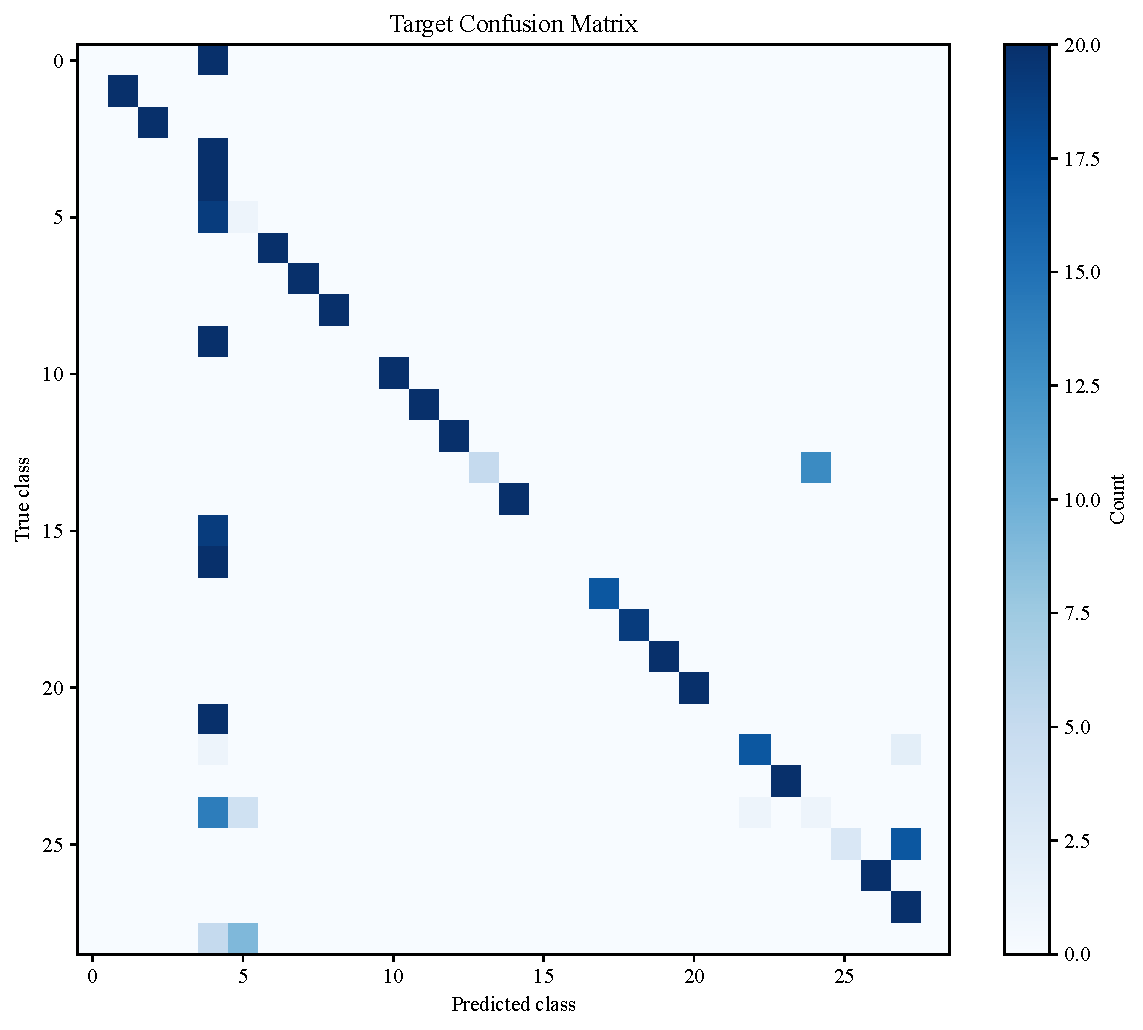
\includegraphics[width=\linewidth,height=0.62\textheight,keepaspectratio]{ch6_multi_sourceonly_5src_to_2_confusion.pdf}\\[-0.05cm]
      \centering{\small SourceOnly\\\textbf{64.02\%}}
    \end{column}
    \begin{column}{0.40\textwidth}
      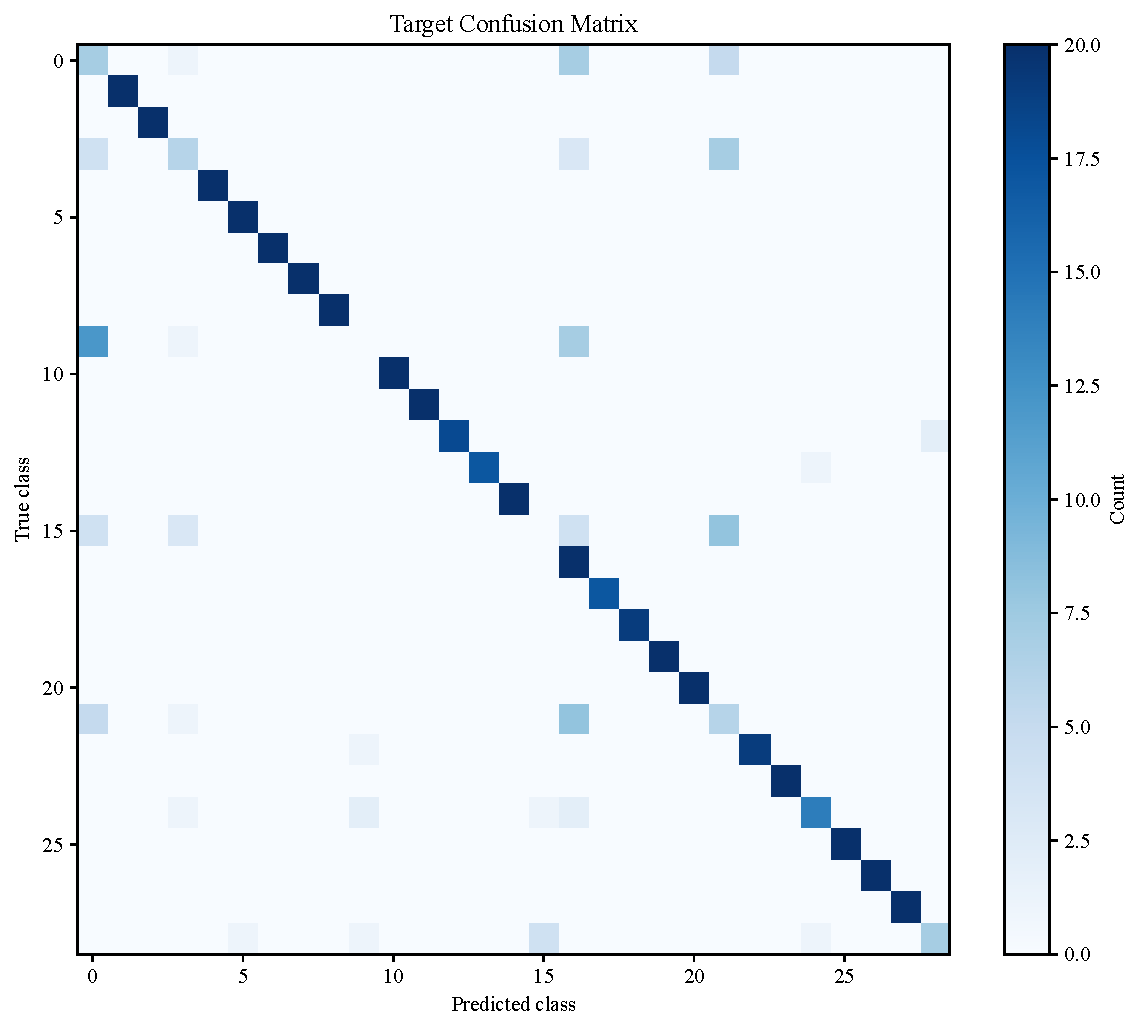
\includegraphics[width=\linewidth,height=0.62\textheight,keepaspectratio]{ch6_multi_CA_CCSR_WJDOT_5src_to_2_confusion.pdf}\\[-0.05cm]
      \centering{\small CA-CCSR-WJDOT\\\textbf{82.89\%}}
    \end{column}
    \begin{column}{0.17\textwidth}
      \vspace{0.55cm}
      \tagpill{blue}{五源输入}\\[0.16cm]
      \tagpill{teal}{逐源传输}\\[0.16cm]
      \tagpill{amber}{类别可靠性}\\[0.45cm]
      {\small\color{muted}多源样本更多，但需要判断每个源域在哪些类别上可靠。}
    \end{column}
  \end{columns}
\end{frame}

\paperref{P48--49}
\begin{frame}{方法三验证：域间融合与类别聚集}
  \begin{columns}[T,totalwidth=\textwidth]
    \begin{column}{0.48\textwidth}
      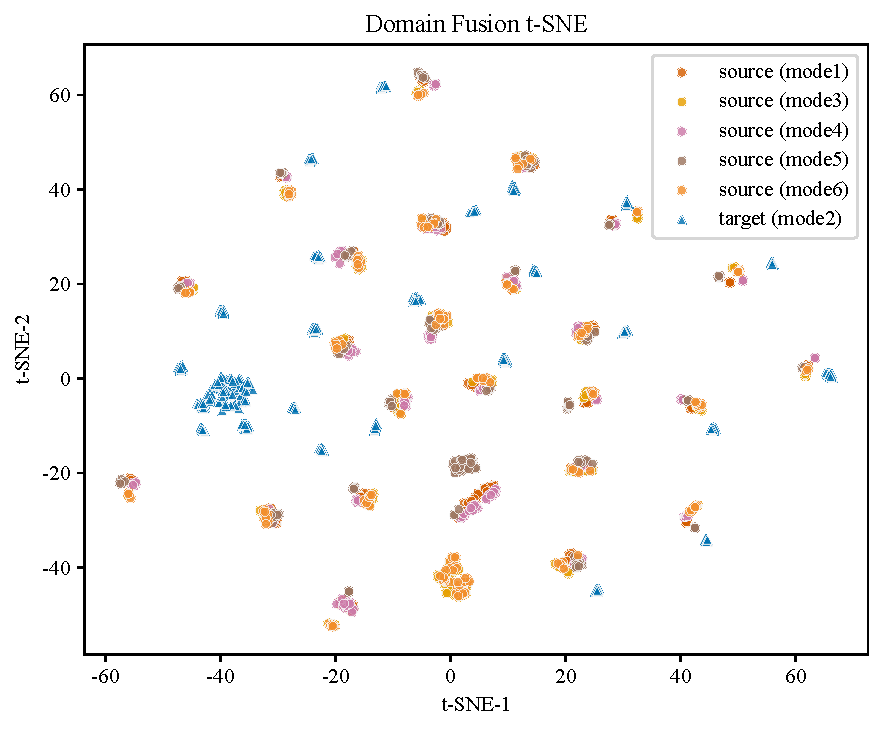
\includegraphics[width=\linewidth,height=0.31\textheight,keepaspectratio]{ch6_multi_sourceonly_5src_to_2_tsne_domain.pdf}
      \captionline{SourceOnly：域 t-SNE}
      \vspace{0.08cm}
      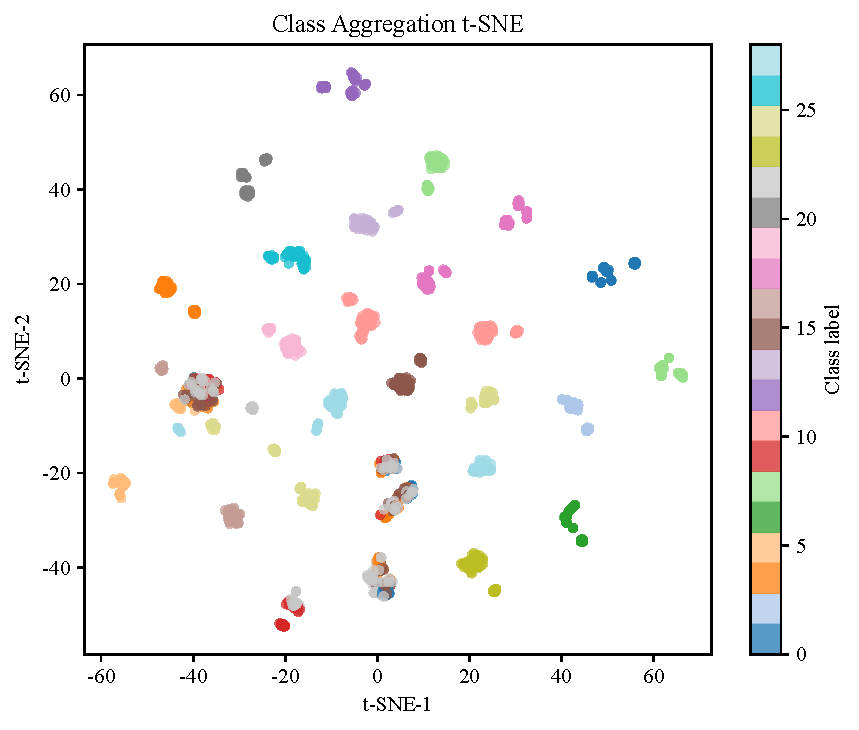
\includegraphics[width=\linewidth,height=0.31\textheight,keepaspectratio]{ch6_multi_sourceonly_5src_to_2_tsne_class.pdf}
      \captionline{SourceOnly：类 t-SNE}
    \end{column}
    \begin{column}{0.48\textwidth}
      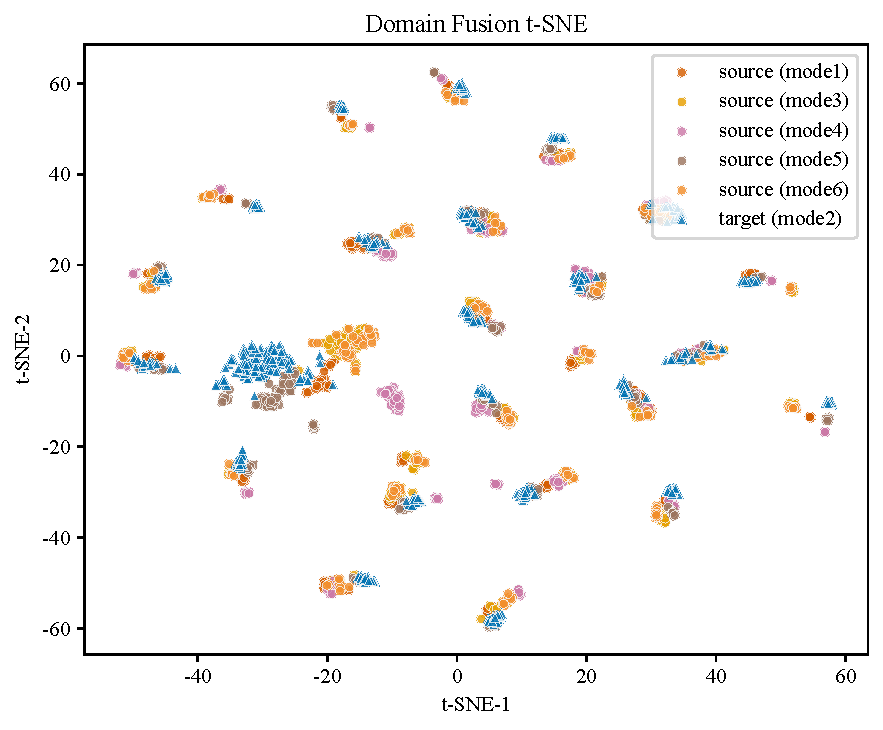
\includegraphics[width=\linewidth,height=0.31\textheight,keepaspectratio]{ch6_multi_CA_CCSR_WJDOT_5src_to_2_tsne_domain.pdf}
      \captionline{CA-CCSR-WJDOT：域 t-SNE}
      \vspace{0.08cm}
      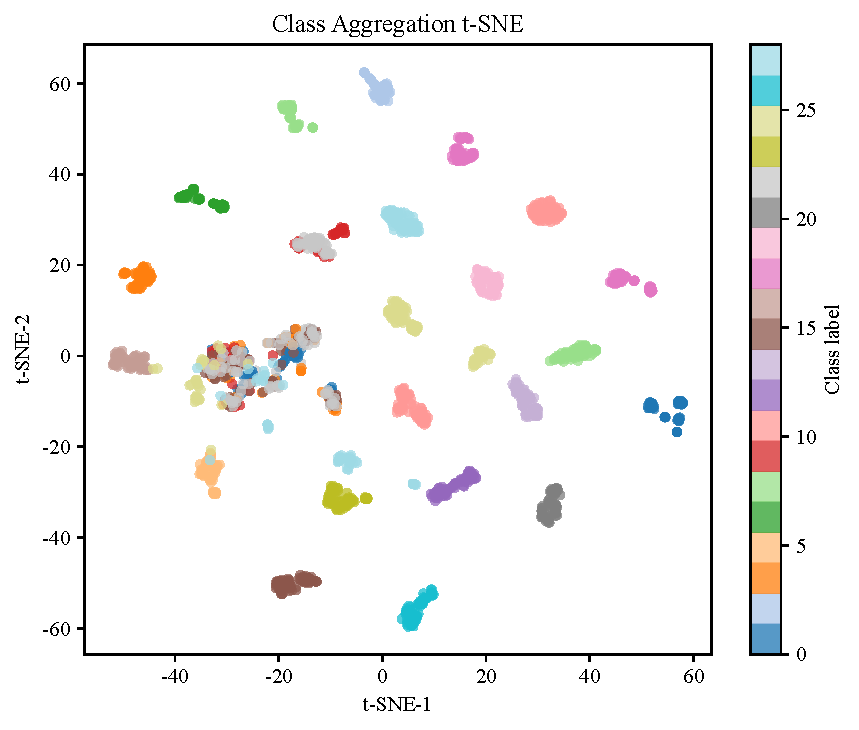
\includegraphics[width=\linewidth,height=0.31\textheight,keepaspectratio]{ch6_multi_CA_CCSR_WJDOT_5src_to_2_tsne_class.pdf}
      \captionline{CA-CCSR-WJDOT：类 t-SNE}
    \end{column}
  \end{columns}
\end{frame}

\paperref{P54}
\begin{frame}{方法三解释：源域--类别权重矩阵}
  \begin{columns}[T,totalwidth=\textwidth]
    \begin{column}{0.56\textwidth}
      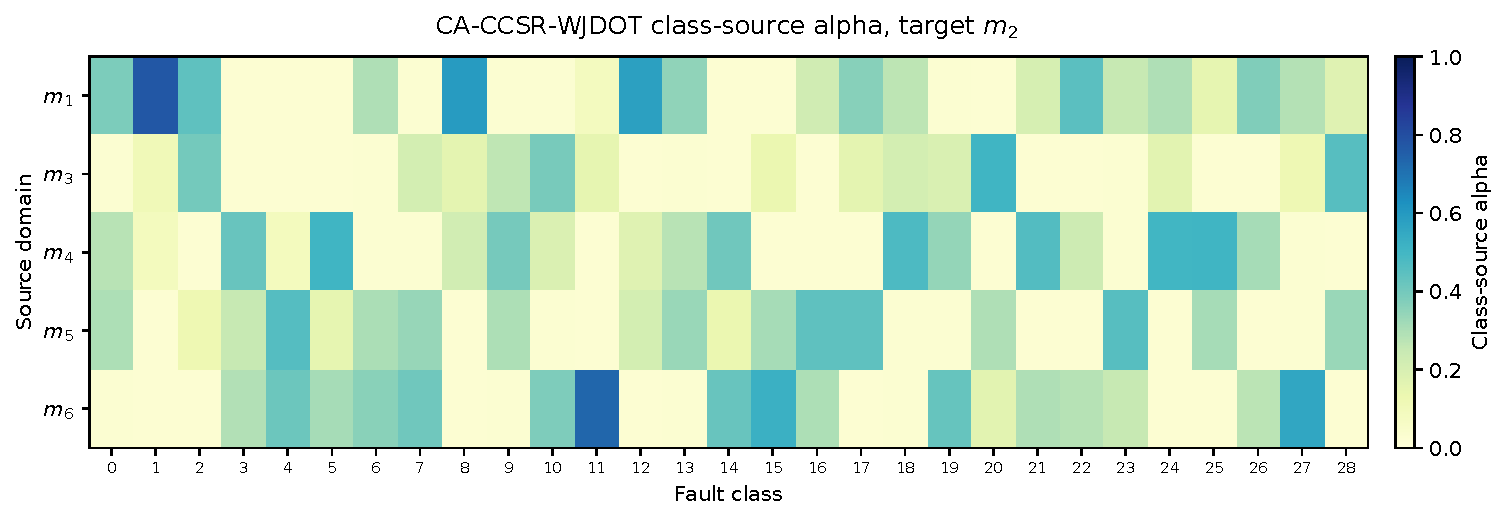
\includegraphics[width=\linewidth,height=0.62\textheight,keepaspectratio]{ch6_class_source_alpha_heatmap.pdf}
      \captionline{五源任务 $\{m_1,m_3,m_4,m_5,m_6\}\rightarrow m_2$}
    \end{column}
    \begin{column}{0.39\textwidth}
      \vspace{0.35cm}
      \metricbox{类别粒度}{不是单一源域权重}{每列重新分配}
      \vspace{0.25cm}

      \metricbox{选择性迁移}{可靠源域贡献更高}{降低负迁移}
      \vspace{0.35cm}

      {\small\color{muted}不同故障类别依赖不同源模式，说明方法不是简单平均多个源域，而是在源域--故障类别层面重新分配迁移贡献。}
    \end{column}
  \end{columns}
\end{frame}

\paperref{P42}
\begin{frame}{实验协议：目标标签仅用于最终评价}
  \begin{columns}[T,totalwidth=\textwidth]
    \begin{column}{0.50\textwidth}
      \small
      \begin{tabular}{lcc}
        \toprule
        实验组 & 规模 & 目的 \\
        \midrule
        单源 & $6\times8$ & 单源递进链 \\
        两源 & $3\times5$ & 小规模多源 \\
        五源 & $6\times5$ & 多源压力测试 \\
        \bottomrule
      \end{tabular}
      \vspace{0.55cm}

      \begin{tikzpicture}[node distance=0.28cm]
        \node[box, fill=blue!7, draw=blue!35, minimum width=5.0cm] (fold) {固定第一折划分};
        \node[box, fill=teal!7, draw=teal!35, below=of fold, minimum width=5.0cm] (targetunlabeled) {目标训练样本无标签};
      \end{tikzpicture}
    \end{column}
    \begin{column}{0.45\textwidth}
      \vspace{0.05cm}
      \metricbox{Accuracy}{整体诊断准确率}{越高越好}
      \hfill
      \metricbox{Macro-F1}{类别等权 F1}{关注少数类}
      \vspace{0.2cm}

      \metricbox{BAcc}{平衡准确率}{类别召回平均}
      \hfill
      \metricbox{t-SNE}{结构证据}{看域与类}
      \vspace{0.25cm}

      {\small\color{red}Target-ref 只作为有标签参考，不参与 UDA 方法排名。}
    \end{column}
  \end{columns}
\end{frame}

\paperref{P50}
\begin{frame}{单源结果：主提升来自对齐，细化来自伪标签}
  \begin{columns}[T,totalwidth=\textwidth]
    \begin{column}{0.50\textwidth}
      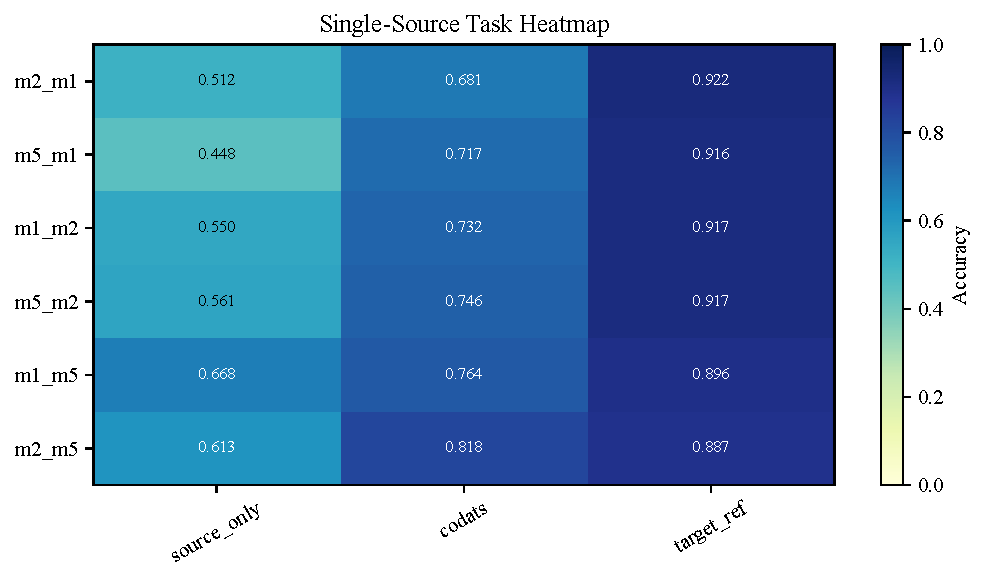
\includegraphics[width=\linewidth,height=0.72\textheight,keepaspectratio]{ch6_single_source_heatmap.pdf}
    \end{column}
    \begin{column}{0.47\textwidth}
      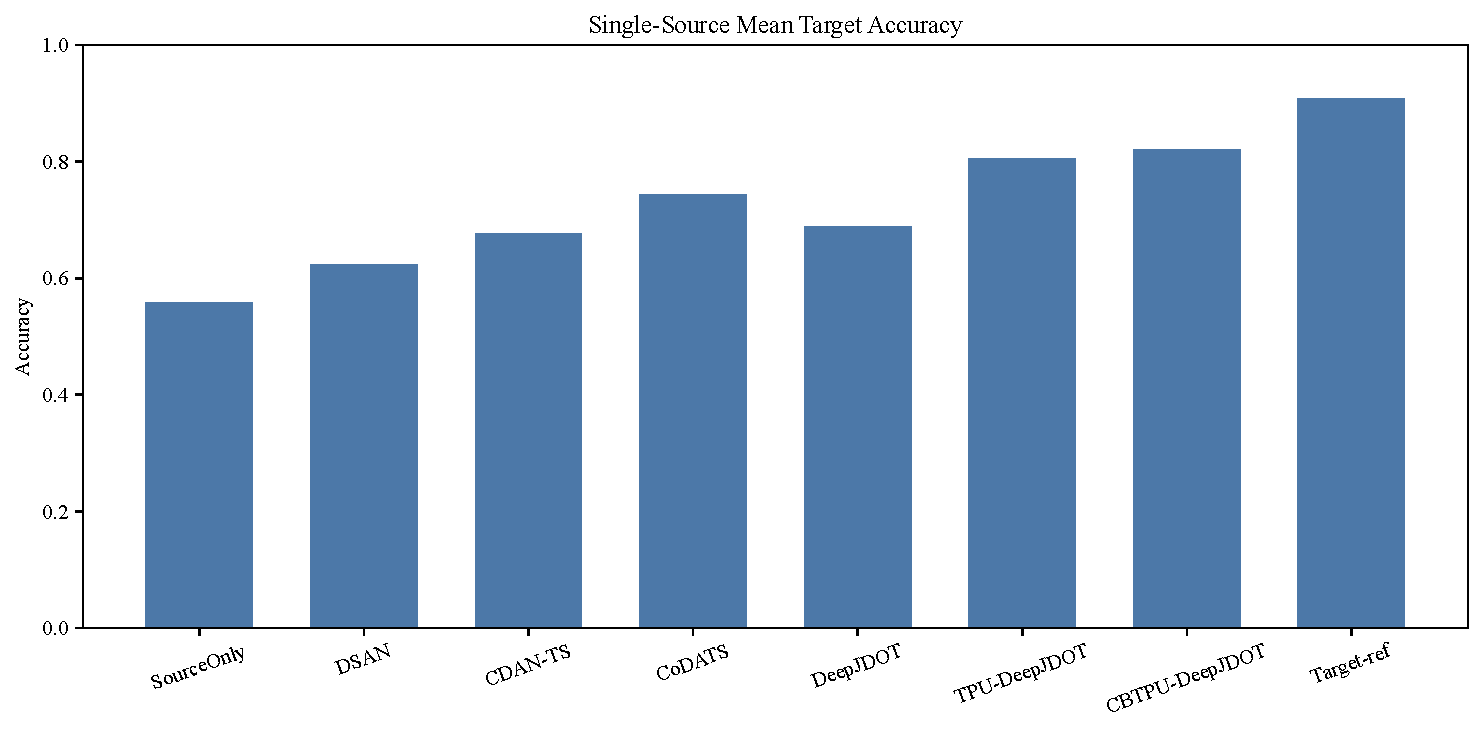
\includegraphics[width=\linewidth,height=0.40\textheight,keepaspectratio]{ch6_single_source_mean_accuracy.pdf}
      \vspace{0.14cm}

      \tinymetric{+11.66}{TPU $\uparrow$ DeepJDOT}{准确率百分点}
      \hfill
      \tinymetric{+1.48}{CBTPU $\uparrow$ TPU}{准确率百分点}
      \hfill
      \tinymetric{82.02\%}{CBTPU}{6/6 第一}
    \end{column}
  \end{columns}
\end{frame}

\paperref{P53}
\begin{frame}{多源结果：类别级可靠性压住负迁移}
  \begin{columns}[T,totalwidth=\textwidth]
    \begin{column}{0.47\textwidth}
      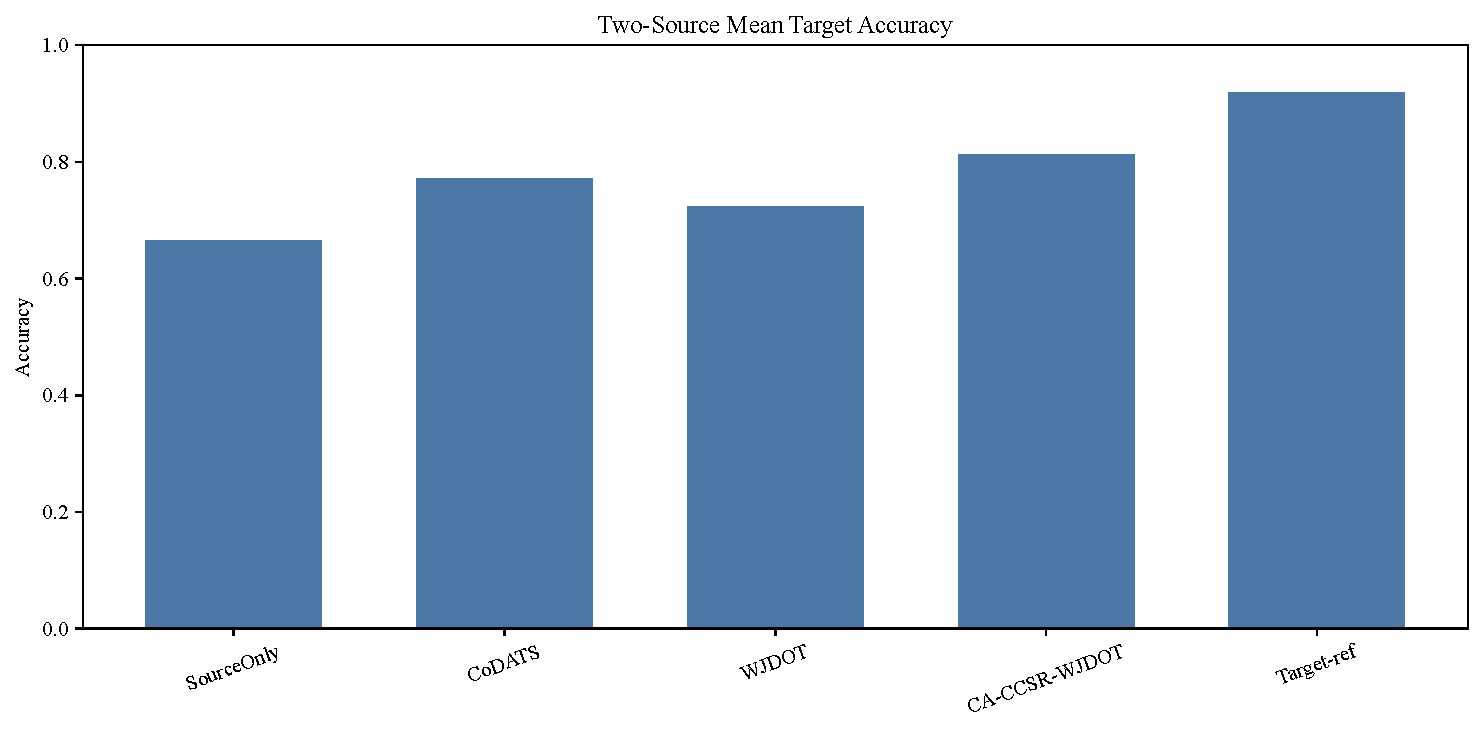
\includegraphics[width=\linewidth,height=0.54\textheight,keepaspectratio]{ch6_two_source_mean_accuracy.pdf}
      \centering{\small 两源：CA-CCSR-WJDOT \textbf{81.21\%}，3/3 第一}
    \end{column}
    \begin{column}{0.47\textwidth}
      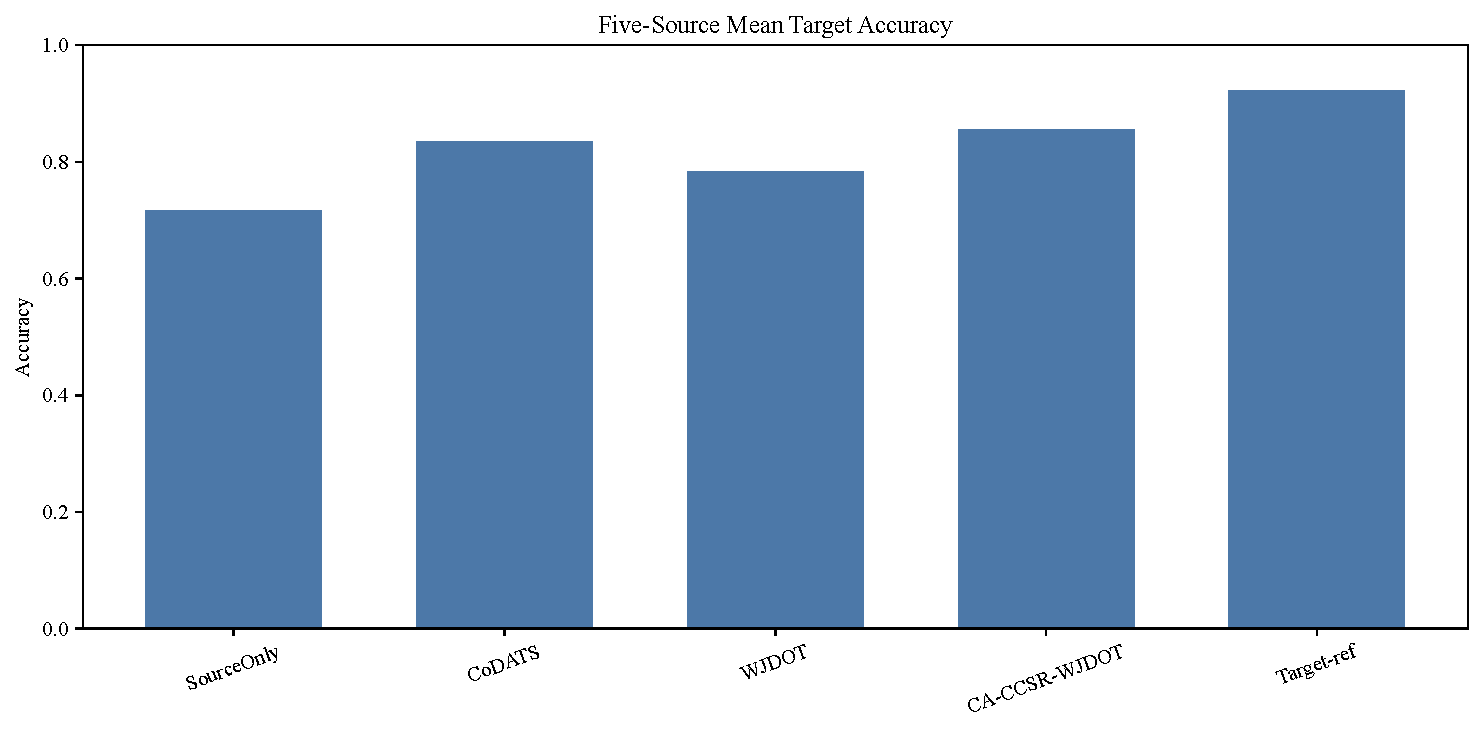
\includegraphics[width=\linewidth,height=0.54\textheight,keepaspectratio]{ch6_five_source_mean_accuracy.pdf}
      \centering{\small 五源：CA-CCSR-WJDOT \textbf{85.50\%}，6/6 第一}
    \end{column}
  \end{columns}
  \vspace{0.25cm}
  \centering
  {\small\color{muted}相对 WJDOT，多源 9 个任务平均准确率提升 7.69 个百分点。}
\end{frame}

\paperref{P54}
\begin{frame}{结论：三类风险对应三类结构约束}
  \centering
  \metricbox{+11.66}{TPU-DeepJDOT $\uparrow$ DeepJDOT}{$p=0.015625$}
  \hfill
  \metricbox{+1.48}{CBTPU-DeepJDOT $\uparrow$ TPU}{$p=0.015625$}
  \hfill
  \metricbox{+7.69}{CA-CCSR-WJDOT $\uparrow$ WJDOT}{$p=0.001953$}

  \vspace{0.65cm}
  \begin{tikzpicture}[node distance=0.45cm]
    \node[box, fill=blue!7, draw=blue!35, minimum width=2.9cm] (a) {样本匹配};
    \node[box, fill=teal!7, draw=teal!35, minimum width=2.9cm, right=of a] (b) {目标筛选};
    \node[box, fill=amber!9, draw=amber!40, minimum width=2.9cm, right=of b] (c) {源域类别分配};
    \draw[arrow] (a) -- (b);
    \draw[arrow] (b) -- (c);
  \end{tikzpicture}

  \vspace{0.35cm}
  {\large\bfseries 跨生产模式故障诊断，需要同时处理这三件事。}
\end{frame}

\paperref{P57}
\begin{frame}{展望}
  \begin{columns}[T,totalwidth=\textwidth]
    \begin{column}{0.48\textwidth}
      \begin{tikzpicture}[node distance=0.28cm]
        \node[box, fill=blue!7, draw=blue!35, minimum width=5.3cm] (fewshot) {少量目标标签预算：1 / 3 / 5 shot};
        \node[box, fill=teal!7, draw=teal!35, below=of fewshot, minimum width=5.3cm] (tta) {连续目标批次测试时自适应};
        \node[box, fill=amber!9, draw=amber!40, below=of tta, minimum width=5.3cm] (matrixperturb) {源域--类别矩阵扰动验证};
      \end{tikzpicture}
    \end{column}
    \begin{column}{0.48\textwidth}
      \begin{tikzpicture}[node distance=0.28cm]
        \node[box, fill=violet!8, draw=violet!40, minimum width=5.3cm] (ablation) {机制裁剪 + 训练效率统计};
        \node[box, fill=red!6, draw=red!35, below=of ablation, minimum width=5.3cm] (robust) {真实现场噪声、缺失、漂移、未知故障};
      \end{tikzpicture}
      \vspace{0.7cm}
      {\small\color{muted}后续重点不是堆叠新模块，而是把有效性、解释性和部署成本继续做成可检验实验。}
    \end{column}
  \end{columns}
\end{frame}

\begin{frame}[plain,noframenumbering]
  \centering
  \vfill
  {\Huge\bfseries 谢谢}
  \vfill
\end{frame}

\end{document}
